\documentclass[11pt,a4paper]{article}

% KAIS initial submission: Springer Nature guidelines (2026) permit common LaTeX style.
% This is a manuscript-review layout, not the historical Elsevier journal class.
% All source sections are in this file; the only external source is references.bib.
% Five original vector PDF figures remain external non-TeX assets.
\usepackage[T1]{fontenc}
\usepackage[utf8]{inputenc}
\usepackage{lmodern}
\usepackage{acronym}
\usepackage{amsmath}
\usepackage{amssymb}
\usepackage{array}
\usepackage{booktabs}
\usepackage{caption}
% Springer Nature KAIS: "Fig. N" captions without a separating colon.
\captionsetup[figure]{name=Fig.,labelfont=bf,labelsep=space,font=small}
\captionsetup[table]{name=Table,labelfont=bf,labelsep=space,font=small}
\usepackage{enumitem}
\usepackage{float}
\usepackage{graphicx}
\usepackage{hyperref}
\usepackage{xurl} % Allow full DOI and dataset URLs to break safely
\usepackage{lineno}
\usepackage{microtype}
\usepackage[numbers,sort&compress]{natbib}
\usepackage[section]{placeins}
\usepackage{tabularx}
\usepackage{xcolor}
% Springer Nature KAIS asks for DOI links in https://doi.org/... form.
% unsrtnat.bst calls \doi; override its fallback 'doi: ...' rendering.
\providecommand{\doi}[1]{\url{https://doi.org/#1}}
\urlstyle{same}

\hypersetup{
 colorlinks=true, linkcolor=blue, citecolor=blue, urlcolor=blue,
 pdftitle={MouseClaimBench: Non-Compensatory Knowledge-Based Authorization of Scientific Claims with Evidence Integrity},
 pdfauthor={Alberto Fernandez-Isabel, Isaac Martin de Diego, Ruben Fuentes-Fernandez},
 pdfsubject={Knowledge-based scientific claim authorization and package integrity},
 pdfkeywords={Knowledge-based systems, Scientific claim authorization, Non-compensatory reasoning, Evidence provenance, Explainable decisions, Computational neuroscience}
}

\acrodef{ach}[ACh]{acetylcholine}
\acrodef{ai}[AI]{Artificial Intelligence}
\acrodef{asp}[ASP]{Answer Set Programming}
\acrodef{bmtk}[BMTK]{Brain Modeling ToolKit}
\acrodef{dandi}[DANDI]{Distributed Archives for Neurophysiology Data Integration}
\acrodef{fair}[FAIR]{Findable, Accessible, Interoperable, and Reusable}
\acrodef{ibl}[IBL]{International Brain Laboratory}
\acrodef{microns}[MICRONS]{Machine Intelligence from Cortical Networks}
\acrodef{nwb}[NWB]{Neurodata Without Borders}
\acrodef{prov}[PROV-O]{PROV Ontology}
\acrodef{rdf}[RDF]{Resource Description Framework}
\acrodef{shacl}[SHACL]{Shapes Constraint Language}
\acrodef{vbn}[VBN]{Visual Behavior Neuropixels}
\acrodef{vone}[V1]{primary visual cortex}
\acrodef{vv}[V\&V]{Verification and Validation}

\setlist[itemize]{leftmargin=*,itemsep=0.45em,topsep=0.45em}
\newcolumntype{Y}{>{\raggedright\arraybackslash}X}
\newcolumntype{P}[1]{>{\raggedright\arraybackslash}p{#1}}
\modulolinenumbers[5]
\setlength{\emergencystretch}{2em}
\setcounter{topnumber}{3}
\setcounter{bottomnumber}{2}
\setcounter{totalnumber}{5}
\renewcommand{\topfraction}{0.92}
\renewcommand{\bottomfraction}{0.80}
\renewcommand{\textfraction}{0.08}
\renewcommand{\floatpagefraction}{0.72}

\makeatletter
\AtBeginDocument{%
  \setlength{\@fptop}{0pt}%
  \setlength{\@dblfptop}{0pt}%
}
\makeatother


\newcommand{\MouseBrainBenchCompanion}{Fern\'andez-Isabel et al., \emph{MouseBrainBench: A Claim-Aware Validation Framework for Partial Mouse-Brain Digital Models}, companion manuscript under review}
\begin{document}

\title{MouseClaimBench: Non-Compensatory Knowledge-Based Authorization of Scientific Claims with Evidence Integrity}
\author{Alberto Fern\'andez-Isabel$^{1,\ast}$ \and Isaac Mart\'in de Diego$^1$ \and Rub\'en Fuentes-Fern\'andez$^2$}
\date{}
\maketitle
\begin{center}
\small
$^1$Data Science Laboratory, Research Centre for Intelligent Information Technologies, Rey Juan Carlos University, M\'ostoles, Madrid, Spain\\
$^2$Institute of Knowledge Technology, Department of Software Engineering and Artificial Intelligence, Complutense University of Madrid, Madrid, Spain\\
$^{\ast}$Correspondence: \href{mailto:alberto.fernandez.isabel@urjc.es}{alberto.fernandez.isabel@urjc.es}
\end{center}
\vspace{1ex}
\begin{abstract}
%% BEGIN ORIGINAL SOURCE: abstract.tex; KAIS-oriented abstract revision (see traceability document).
Scientific information systems integrate heterogeneous experimental, computational, and provenance artifacts, but successful prediction or reproducible workflows do not justify arbitrary mechanistic or causal claims. We authorize bounded scientific claims against explicit, versioned evidence requirements rather than estimating scientific truth. MouseClaimBench implements three non-compensatory gates for domain evidence, structural conformance, and relational package integrity, returning category-complete deficits with artifact-level witnesses. An author-defined mouse-brain profile specifies 10 claim types, 22 predicate contracts, 60 claim--evidence requirements, and 124 observation slots; its content has not been independently validated. The architecture combines independently implemented Python and Answer Set Programming authorization, RDF/PROV-O and JSON-LD interchange, and external SHACL graph validation. Across 5,677 controlled contract cases, Python and ASP agree on domain decisions and deficits; 55,031 deterministic property checks reveal no violations. All 2,550 evaluated attack-composition packages are rejected, whereas 20 internally coherent forgeries demonstrate the absence of an external trust anchor. Two pre-access-frozen DANDI protocols yield one availability refusal and one bounded predictive authorization for 32 mice; a MICRONS application supports only a local observational association. These results establish reproducible, profile-relative knowledge-based authorization and characterize its integrity boundary, without establishing biological truth, expert consensus, or generality beyond the evaluated domain.
%% END ORIGINAL SOURCE: abstract.tex (revised)
\end{abstract}

\noindent\textbf{Keywords:} Knowledge-based systems; Scientific claim authorization; Non-compensatory reasoning; Evidence provenance; Explainable decisions; Computational neuroscience.
\vspace{1.5ex}

\linenumbers
\acresetall


%% BEGIN ORIGINAL SOURCE: introduction.tex (SHA256 503b2fcfec6935bec6628819e47f89faadcb8a0cc624bf6c1693cdd232ef97f2)
\section{Introduction}
\label{sec:introduction}

Artificial Intelligence systems increasingly operate over heterogeneous
scientific evidence produced by predictive models, simulations, experimental
datasets, statistical analyses, and computational workflows. A central
difficulty is that the evidential meaning of these artifacts depends on the
claim being assessed. Accurate prediction may support a bounded predictive
claim without identifying the mechanism that generated the observations.
Reproducible execution does not imply independent scientific replication, and
an observational association does not establish causality. An intelligent
decision-support system that reasons over scientific evidence must therefore
distinguish not only whether evidence is present, but also which claims that
evidence is entitled to support.

This work formulates this problem as \emph{scientific claim authorization}.
Given a bounded claim, a declared evidence policy, and a package of scientific
artifacts, the task is to determine whether the available evidence satisfies
all requirements associated with that claim and, when it does not, to return
the complete set of violated requirements. This differs from predicting the
truth of a proposition or assigning a global quality score to an experiment.
The decision is policy-relative and non-compensatory: strong evidence for one
requirement cannot replace missing or inadmissible evidence for another.
Such a formulation is particularly relevant for intelligent systems that must
produce auditable decisions from heterogeneous evidence rather than a single
learned score.

Computational neuroscience provides a demanding application for this problem
because its public resources span substantially different biological scales,
experimental designs, and computational objectives. Allen tracer experiments
describe mesoscale connectivity, population recordings characterize behavior
and neural response, Sensorium benchmarks assess predictive performance, and
\ac{microns} links anatomical and functional measurements inside a restricted
cortical volume
\citep{oh2014mesoscale,willeke2022sensorium,turishcheva2023dynamic,bae2025microns}.
The Virtual Mouse Brain, \ac{bmtk}, and detailed models of mouse primary
visual cortex provide established simulation capabilities
\citep{melozzi2017virtualmouse,dai2020bmtk,billeh2020v1}. Digital Twin Brain
proposals extend this landscape through data assimilation and multiscale
modeling \citep{xiong2023dtb,chen2026mousedtb}. These resources provide
valuable but non-equivalent forms of evidence. Treating prediction,
reproducibility, topology, intervention, anatomical coverage, and provenance
as interchangeable signals can therefore authorize interpretations that are
stronger than the evidence supports.

Existing scientific claim verification systems primarily retrieve documentary
evidence and classify whether passages, tables, or figures support a
proposition
\citep{wadden2020scifact,wadden2022multivers,lu2023scitab,wang2025sciver}.
Recent benchmarks also evaluate the extraction and linkage of claim--evidence
pairs from complete scientific articles \citep{javaji2025claimbench}.
Knowledge-based systems and assurance approaches provide explicit
representations of claims, evidence, rules, and argument structures
\citep{buchanan1984rulebased,studer1998knowledge,mohamad2021assurance},
while \ac{prov} and \ac{shacl} provide standardized mechanisms for provenance
representation and graph validation
\citep{lebo2013provo,w3c2017shacl}. These approaches address complementary
parts of the problem, but none of them alone determines whether a structured
scientific evidence package satisfies the complete set of claim-specific
scientific, structural, and integrity requirements required for authorization.

We introduce MouseClaimBench, an integrity-aware intelligent system for
scientific claim authorization. MouseClaimBench represents claim-specific
evidence requirements in a versioned knowledge profile and evaluates an
evidence package through three logically distinct dimensions. Domain
authorization determines whether every mandatory evidence block satisfies its
declared scientific predicate. Structural conformance determines whether the
required data and relations are represented correctly. Package integrity
determines whether artifact identity, hashes, derivations, attestations,
independence declarations, and cohort relations are internally coherent.
Final authorization is granted only when all three dimensions pass.

This separation enables a non-compensatory form of symbolic decision making.
Predictive performance cannot compensate for missing topology evidence,
structural completeness cannot compensate for a failed scientific predicate,
and an otherwise sufficient evidence package cannot compensate for incoherent
provenance. When authorization fails, MouseClaimBench preserves every
violated deficit category and an actionable witness rather than returning a
single prioritized explanation or aggregate score. The resulting decision is
therefore reproducible, inspectable, and attributable to an explicit
knowledge policy.

\noindent\textbf{Research contributions.}\label{sec:contributions}\par
The paper makes the following contributions:
\begin{itemize}

    \item A formalization of scientific claim authorization as a
    profile-relative, non-compensatory decision problem over heterogeneous
    scientific evidence, with explicit separation of domain authorization,
    structural conformance, and package integrity.

    \item An executable knowledge representation comprising 10 bounded
    claims, 22 predicate contracts, 60 claim--evidence relations, and 124
    required observation slots. Each relation has a stable identifier,
    claim-specific necessity rationale, scope, exceptions, sources, and
    explicit policy status.

    \item An integrity-aware reasoning architecture that combines a primary
    Python authorization engine, a separately implemented \ac{asp} reasoning
    path, and interoperable \ac{rdf}/\ac{prov} and JSON-LD representations
    validated externally through \ac{shacl}.

    \item A category-complete explanation mechanism in which authorization
    failures retain all violated requirement classes and their actionable
    witnesses, together with counterfactual verification of explanation
    sufficiency and individual necessity.

    \item A systematic verification strategy combining property-based
    testing, one-edge policy perturbation, controlled integrity attacks,
    leave-one-control-out ablations, extended regression tests, and
    coherent-forgery controls to characterize implementation conformance and
    the system's explicit trust boundary.

    \item Artifact-grounded evaluation on computational mouse-brain resources,
    including two \ac{dandi}/\ac{nwb} protocols frozen before numerical asset
    access and a dependence-aware \ac{microns} analysis, demonstrating both
    bounded authorization and refusal under unchanged decision rules.

\end{itemize}

The methodological contribution is the formulation and executable realization
of claim authorization as an auditable intelligent-system decision process
over heterogeneous scientific artifacts. Existing techniques for rule-based
reasoning, provenance representation, and graph validation are used as
components of this architecture, while the contribution lies in how
claim-specific scientific semantics, structural requirements, relational
integrity, non-compensatory reasoning, and category-complete explanations are
jointly represented, executed, and evaluated. The current empirical study
focuses on computational mouse-brain evidence; broader domain generality
therefore remains an architectural capability rather than an empirical claim.

The evaluation is organized around three research questions: (RQ1) whether the independent reasoning and validation paths implement the same declared authorization contracts; (RQ2) whether the integrity controls reject the specified package attacks without masking distinct deficit categories, and where the trust boundary remains; and (RQ3) whether the same profile-relative decision rules yield appropriately bounded authorizations and refusals for public scientific artifacts. These questions concern the behavior of the specified knowledge system, not independent truth or consensus validity of its author-defined scientific policy.

This formulation does not claim novelty in rule engines, assurance cases, provenance vocabularies, or graph-validation standards in isolation. The evaluated unit is instead a claim-conditioned knowledge-system decision with non-interchangeable scientific, graph, and relational-integrity obligations, a complete set of failed obligations, and explicit negative controls. The current evidence establishes conformance and controlled robustness relative to this policy; it does not demonstrate that the policy is optimal or transferable without domain-specific knowledge acquisition.

The remainder of the paper is organized as follows.
Section~\ref{sec:related-work} positions MouseClaimBench with respect to
scientific claim verification, intelligent and knowledge-based systems,
assurance reasoning, semantic validation, provenance, and computational
neuroscience. Section~\ref{sec:method} defines the authorization model and
execution architecture. Section~\ref{sec:experiments} presents the experimental
evaluation. Section~\ref{sec:discussion} discusses the results, scope, and
limitations. Finally, Section~\ref{sec:conclusions} summarizes the conclusions
and future research directions.
%% END ORIGINAL SOURCE: introduction.tex



%% BEGIN ORIGINAL SOURCE: related_work.tex (SHA256 635dfabfdf2237eada131fe202c7676559342755e232ef56ce151f13b377a674)
\section{Related Work and Methodological Positioning}
\label{sec:related-work}

Scientific claim authorization intersects several established research areas:
scientific claim verification, intelligent and knowledge-based systems,
assurance reasoning, semantic validation, provenance, reproducibility, and
computational model assessment. These areas address complementary aspects of
evidence-based reasoning, but they differ in their primary decision objects,
the representations over which they reason, and the outputs they produce.
Table~\ref{tab:related-work-v2} compares the closest methodological families
by their primary decision object, evidence representation, treatment of
provenance or integrity, and resulting decision output. The comparison is
intended to clarify the distinct reasoning problem addressed by
MouseClaimBench rather than to rank the approaches.



%% BEGIN ORIGINAL SOURCE: related_work_comparison_v2.tex (SHA256 12fb4c39e037b7c24d6d4f5a7c2f7d0ff344ad9b6a9d8ab0dde27a93b87a0841)
\begin{table}[!htbp]
\centering
\caption{Decision-object comparison with the methodological families closest to MouseClaimBench}
\label{tab:related-work-v2}
\scriptsize
\setlength{\tabcolsep}{2pt}
\renewcommand{\arraystretch}{0.95}

\begin{tabularx}{\textwidth}{
@{}
P{0.16\textwidth}
P{0.19\textwidth}
P{0.21\textwidth}
P{0.16\textwidth}
Y
@{}}
\toprule
Family &
Decision object &
Representation / reasoning &
Integrity / provenance &
Output \\
\midrule

Scientific claim verification
\citep{wadden2020scifact,wadden2022multivers}
&
Support or contradiction of a scientific claim
&
Documentary or multimodal evidence
&
Source traceability
&
Verification label
\\

Rule-based expert systems
\citep{buchanan1984rulebased,studer1998knowledge}
&
Domain inference from explicit knowledge
&
Knowledge bases and symbolic rules
&
Domain-dependent
&
Rule-derived conclusion
\\

Assurance cases
\citep{batarseh2021assurance,mohamad2021assurance}
&
Justification of a system property
&
Claims, arguments, assumptions, and evidence
&
Explicit evidence relations
&
Assurance argument
\\

\ac{shacl} and \ac{prov}
\citep{lebo2013provo,w3c2017shacl}
&
Graph conformance and provenance
&
Shapes, constraints, and derivations
&
Primary concern
&
Validation report / provenance graph
\\

Model \ac{vv} and reproducibility
\citep{asme2018vv40,pineau2021reproducibility}
&
Credibility and empirical adequacy
&
Metrics, uncertainty, and protocols
&
Traceability and reproducibility
&
Validation assessment
\\

Neural model benchmarks
\citep{willeke2022sensorium,turishcheva2023dynamic}
&
Performance on a defined task
&
Dataset-specific metrics
&
Benchmark-specific
&
Task-specific result
\\

MouseClaim\allowbreak{}Bench
&
Authorization of a bounded scientific claim
&
Versioned profile and symbolic requirements
&
Structural and relational integrity
&
Non-compensatory authorization with deficit traces
\\

\bottomrule
\end{tabularx}
\end{table}
%% END ORIGINAL SOURCE: related_work_comparison_v2.tex




\subsection{Scientific claim verification and intelligent systems}
\label{subsec:claims-assurance}

Scientific claim verification commonly decomposes the task into evidence
retrieval, evidence selection, and support or contradiction classification
\citep{vladika2023survey}. SciFact introduced expert-written claims grounded
in scientific abstracts, while MultiVerS and SciFact-Open extended
full-document and open-domain reasoning
\citep{wadden2020scifact,wadden2022multivers,wadden2022scifactopen}.
SciTab, SciVer, SciTrue, PhyVer, and later multimodal approaches incorporate
tables, figures, physical measurements, and richer evidence paths
\citep{lu2023scitab,wang2025sciver,tan2026scitrue,chen2026phyver,zhang2026mever}.
CLAIM-BENCH evaluates the extraction and linkage of claim--evidence pairs by
language models \citep{javaji2025claimbench}.

These approaches primarily ask whether retrieved documentary or multimodal
content supports a proposition. MouseClaimBench addresses a different
decision problem. It assumes that scientific evidence artifacts and their
associated predicates have already been produced and asks whether their
scientific type, status, provenance, and relations satisfy all requirements of
a declared claim-specific authorization policy. Consequently, documentary
support cannot substitute for evidence of intervention, independent
replication, topology, anatomical coverage, or another requirement explicitly
associated with the target claim.

Rule-based expert systems provide the classical separation between domain
knowledge, facts, inference procedures, and explanations
\citep{buchanan1984rulebased,studer1998knowledge}. MouseClaimBench follows
this symbolic reasoning tradition but makes the authorization object explicit:
knowledge is represented as a versioned claim profile, scientific artifacts are
represented as typed evidence, and the inference result is a
non-compensatory authorization decision together with the complete set of
violated requirement categories.

Selective prediction also addresses when a prediction should not be issued,
but does so through a learned reject option \citep{geifman2019selectivenet}.
MouseClaimBench instead applies explicit symbolic requirements and does not
learn an abstention threshold. Its refusal decision follows directly from
claim-specific evidence requirements and preserves the requirements that
prevent authorization.

Classical validation of expert and knowledge-based systems distinguishes
implementation correctness from the validity of acquired domain knowledge
\citep{benbasat1989validation,knauf2002validation}. That distinction is
retained here. Multiple execution paths, property tests, and counterfactual
checks can establish whether an implementation follows the declared profile,
but they do not establish that the profile constitutes a complete or
universally accepted scientific ontology.


\subsection{Assurance reasoning and auditable decisions}
\label{subsec:assurance}

Assurance cases organize claims, arguments, assumptions, defeaters, and
evidence for a defined context of use
\citep{batarseh2021assurance,mohamad2021assurance}. More recent work studies
assurance cases as attributed graphs and analyzes structural and
provenance-related differences between human- and machine-generated
arguments \citep{ikhwantri2026assurancegraphs}. Compliance-by-construction
argument graphs combine typed arguments, deterministic admissibility
constraints, and PROV-aligned ledgers for AI-assisted certification records
\citep{moghaddam2026compliance}. Claim-level auditability has similarly been
proposed for research agents through persistent provenance and protocolized
validation \citep{rasheed2026auditability}.

MouseClaimBench shares the objective of auditable evidence-based reasoning,
but its decision object differs from an assurance argument. It does not
construct or score an argument graph. Instead, it executes a declared
claim-specific evidence contract over pre-existing scientific artifacts and
returns either authorization or refusal under that profile. Refusal retains all
detected deficit categories and their corresponding witnesses rather than one
prioritized reason. Explanation is therefore part of the executable decision
semantics rather than a post-hoc summary of the result.


\subsection{Semantic validation, provenance, and reproducibility}
\label{subsec:semantic-standards}

\ac{shacl} validates an \ac{rdf} data graph against a shapes graph and
returns a machine-readable validation report \citep{w3c2017shacl}.
\ac{prov} represents entities, activities, agents, and derivation relations for
interoperable provenance \citep{lebo2013provo}. MouseClaimBench uses both
standards to represent versioned profiles, evidence packages, artifact
relations, and decisions. Profile definitions and evidence packages are
exported as \ac{rdf}/JSON-LD, while an external \ac{shacl} engine checks
structural field and relation constraints.

Structural validity, however, is insufficient for scientific authorization. A
syntactically valid graph can reference the wrong profile, reuse the same
artifact as supposedly independent evidence, declare overlapping cohorts as
disjoint, contain inconsistent attestations, or correctly represent a
scientifically failed evidence block. MouseClaimBench therefore separates
graph conformance from relational package integrity and from domain
authorization. This separation allows a package to be structurally valid
while remaining scientifically unauthorized, or scientifically complete while
failing integrity requirements.

Reproducibility guidance, \ac{fair} principles, model cards, datasheets, and
research-software standards improve disclosure, traceability, and reuse
\citep{nasem2019reproducibility,wilkinson2016fair,mitchell2019modelcards,
gebru2021datasheets,pineau2021reproducibility,barker2022fair4rs}.
\ac{nwb} provides a shared data representation for neurophysiology and
supports reuse through \ac{dandi} \citep{rubel2022nwb}. MouseClaimBench
complements these practices by making resource versions, artifact identities,
official hashes, code revisions, protocol identities, derivations, and bounded
interpretations part of the authorization trace. It also distinguishes clean
computational reproduction, within-resource reproduction, and external study
replication rather than allowing these evidential roles to be treated as
interchangeable.

Model \ac{vv} and uncertainty-quantification frameworks assess
implementation correctness, empirical adequacy, uncertainty, credibility, and
context of use
\citep{oberkampf2010verification,sargent2013verification,asme2018vv40,
riedmaier2021vvuq}. MouseClaimBench consumes the resulting measurements
and validation outcomes as typed evidence rather than replacing these
frameworks. Its role is to prevent success on one validation dimension from
authorizing a claim whose other required evidence is absent or inadmissible.


\subsection{Scientific authorization in computational mouse-brain research}
\label{subsec:mouse-boundaries}

Computational mouse-brain resources provide a demanding application for
claim-specific authorization because their evidence spans different biological
scales, experimental designs, and scientific objectives. Allen tracer data and
derived connectomes support mesoscale structural analysis
\citep{oh2014mesoscale,knox2019connectome}. Sensorium and Dynamic
Sensorium evaluate neural-response prediction under static and video stimuli
\citep{willeke2022sensorium,turishcheva2023dynamic,
turishcheva2024retrospective}. Recent work extends predictive generalization
and analyzes population-response geometry in visual-cortex digital twins, but
predictive performance alone does not uniquely identify a biological
mechanism \citep{wang2025foundation,liscai2025population}.

\ac{microns} combines detailed anatomical and functional measurements in
mouse visual cortex and supports local structure--function analysis
\citep{bae2025microns,ding2025wiring}. Its measurements nevertheless cover
a restricted cortical volume rather than a measured synaptic connectome of the
complete mouse brain. The Virtual Mouse Brain, \ac{bmtk}, and detailed
\ac{vone} models provide simulation and network-construction capabilities at
different scales
\citep{melozzi2017virtualmouse,dai2020bmtk,billeh2020v1}.
Observational causal-direction benchmarks further illustrate that causal
direction requires assumptions beyond association \citep{mooij2016cause}.
Digital Twin Brain and MouseDTB proposals motivate additional distinctions
among prediction, topology, direction, intervention, entity specificity,
anatomical coverage, and operational updating
\citep{xiong2023dtb,chen2026mousedtb}.

These distinctions make computational neuroscience an informative
application domain for scientific claim authorization. MouseClaimBench treats
the outputs of predictive models, simulations, anatomical analyses, statistical
tests, and reproducibility procedures as heterogeneous evidence objects rather
than as interchangeable quality indicators. Authorization is determined from
the requirements of the target claim rather than from a global score.


\subsection{Relationship to the MouseBrainBench validation study}
\label{subsec:mousebrainbench-relationship}

MouseClaimBench follows the MouseBrainBench validation study
(\MouseBrainBenchCompanion), but addresses a different
decision problem. MouseBrainBench evaluates whether model-evaluation
evidence supports bounded interpretations through validation dimensions,
diagnostic measures, and non-compensatory model-assessment criteria. It
includes synthetic systems and bounded Allen, Sensorium, \ac{ibl}, and
\ac{microns} cases.

The present work instead formalizes authorization over a versioned
heterogeneous evidence package. Five frozen MouseBrainBench result packages
are reused only as retrospective authorization inputs and are not counted as
new external validation. The knowledge profile, admissibility semantics,
category-complete authorization, relational integrity model, separately
implemented reasoning paths, controlled integrity evaluation, and prospective
\ac{dandi} protocols are evaluated in the present study. The
dependence-aware \ac{microns} reanalysis extends uncertainty treatment within
the same tissue volume and remains internal reproduction.

Table~\ref{tab:mousebrainbench-relationship} summarizes the distinction
between the two studies in terms of decision object, evidence representation,
reasoning model, integrity treatment, and evaluation design.



%% BEGIN ORIGINAL SOURCE: mousebrainbench_relationship.tex (SHA256 97f3ed4a3994e1a14cee41423881e7dd3d11a531cbcc7662498463f8c1ea4962)
\begin{table}[!htbp]
\centering
\caption{Relationship between MouseBrainBench and MouseClaimBench. Five frozen MouseBrainBench packages are reused only as retrospective authorization inputs}
\label{tab:mousebrainbench-relationship}
\scriptsize
\setlength{\tabcolsep}{4pt}
\renewcommand{\arraystretch}{0.95}

\begin{tabularx}{\textwidth}{
@{}
P{0.19\textwidth}
P{0.36\textwidth}
Y
@{}}
\toprule
Aspect &
MouseBrainBench &
MouseClaimBench \\
\midrule

Decision object
&
Support for bounded interpretations from model-evaluation evidence
&
Authorization of bounded claims from heterogeneous evidence packages
\\

Representation
&
Validation dimensions, evidence contracts, and diagnostic measures
&
10 claims, 22 predicates, 60 claim--evidence requirements, and typed blocks
\\

Reasoning
&
Claim-aware validation with a non-compensatory gate
&
Profile-relative symbolic authorization with complete deficit traces
\\

Standards
&
Not a central evaluated layer
&
\ac{rdf}/\ac{prov}, JSON-LD, \ac{shacl}, and graph-isomorphism checks
\\

Integrity
&
Reproducibility and artifact controls
&
13 relational integrity-deficit types
\\

Execution
&
Original benchmark implementations
&
Python, separate \ac{asp} reasoning, and external \ac{shacl}
\\

Robustness
&
Not a primary objective
&
Controlled attacks, ablations, regressions, and coherent forgeries
\\

External evaluation
&
Retrospective public-resource evaluation
&
Five retrospective mappings, two frozen \ac{dandi} protocols, and \ac{microns}
\\

\bottomrule
\end{tabularx}
\end{table}
%% END ORIGINAL SOURCE: mousebrainbench_relationship.tex



The distinction between the two studies is therefore one of decision object as
well as implementation. MouseBrainBench evaluates the support provided by
specific model-validation results; MouseClaimBench evaluates whether a
versioned package of heterogeneous evidence satisfies the complete
authorization contract associated with a bounded scientific claim. The latter
requires explicit reasoning over scientific admissibility, structural
conformance, and relational integrity and preserves all detected authorization
deficits in the resulting decision trace.
%% END ORIGINAL SOURCE: related_work.tex



%% BEGIN ORIGINAL SOURCE: method.tex (SHA256 e1c48113bb5895a36ee008930c230a17412beaadf8f4e2b4d63bc92b5294e3b5)
\section{Knowledge-Based Authorization: Formal Model and Architecture}
\label{sec:method}

MouseClaimBench implements scientific claim authorization as a symbolic
reasoning process over a versioned knowledge profile, typed evidence blocks,
and a manifest of the scientific artifacts from which those blocks were
derived. Given a bounded claim and an evidence package, the system produces a
profile-relative authorization decision together with layer-resolved deficit
traces and provenance-linked explanations.

The reasoning architecture separates three dimensions that represent
different failure modes: domain authorization, structural conformance, and
package integrity. Domain authorization determines whether the scientific
evidence required by a claim is admissible. Structural conformance determines
whether the required information and relations are represented correctly.
Package integrity evaluates whether provenance, artifact identity,
attestations, and declared independence relations are internally coherent.
The separation is intentional: a structurally valid graph can contain
incoherent provenance, and an internally coherent package can still lack the
scientific evidence required by the target claim.
Fig.~\ref{fig:standards-workflow} summarizes the complete architecture.



%% BEGIN ORIGINAL SOURCE: standards_workflow.tex (SHA256 228a33a285997ae584c8f8d3c7a64e125a1eed04d2257858107d82334ad45c92)
\begin{figure}[!htbp]
\centering
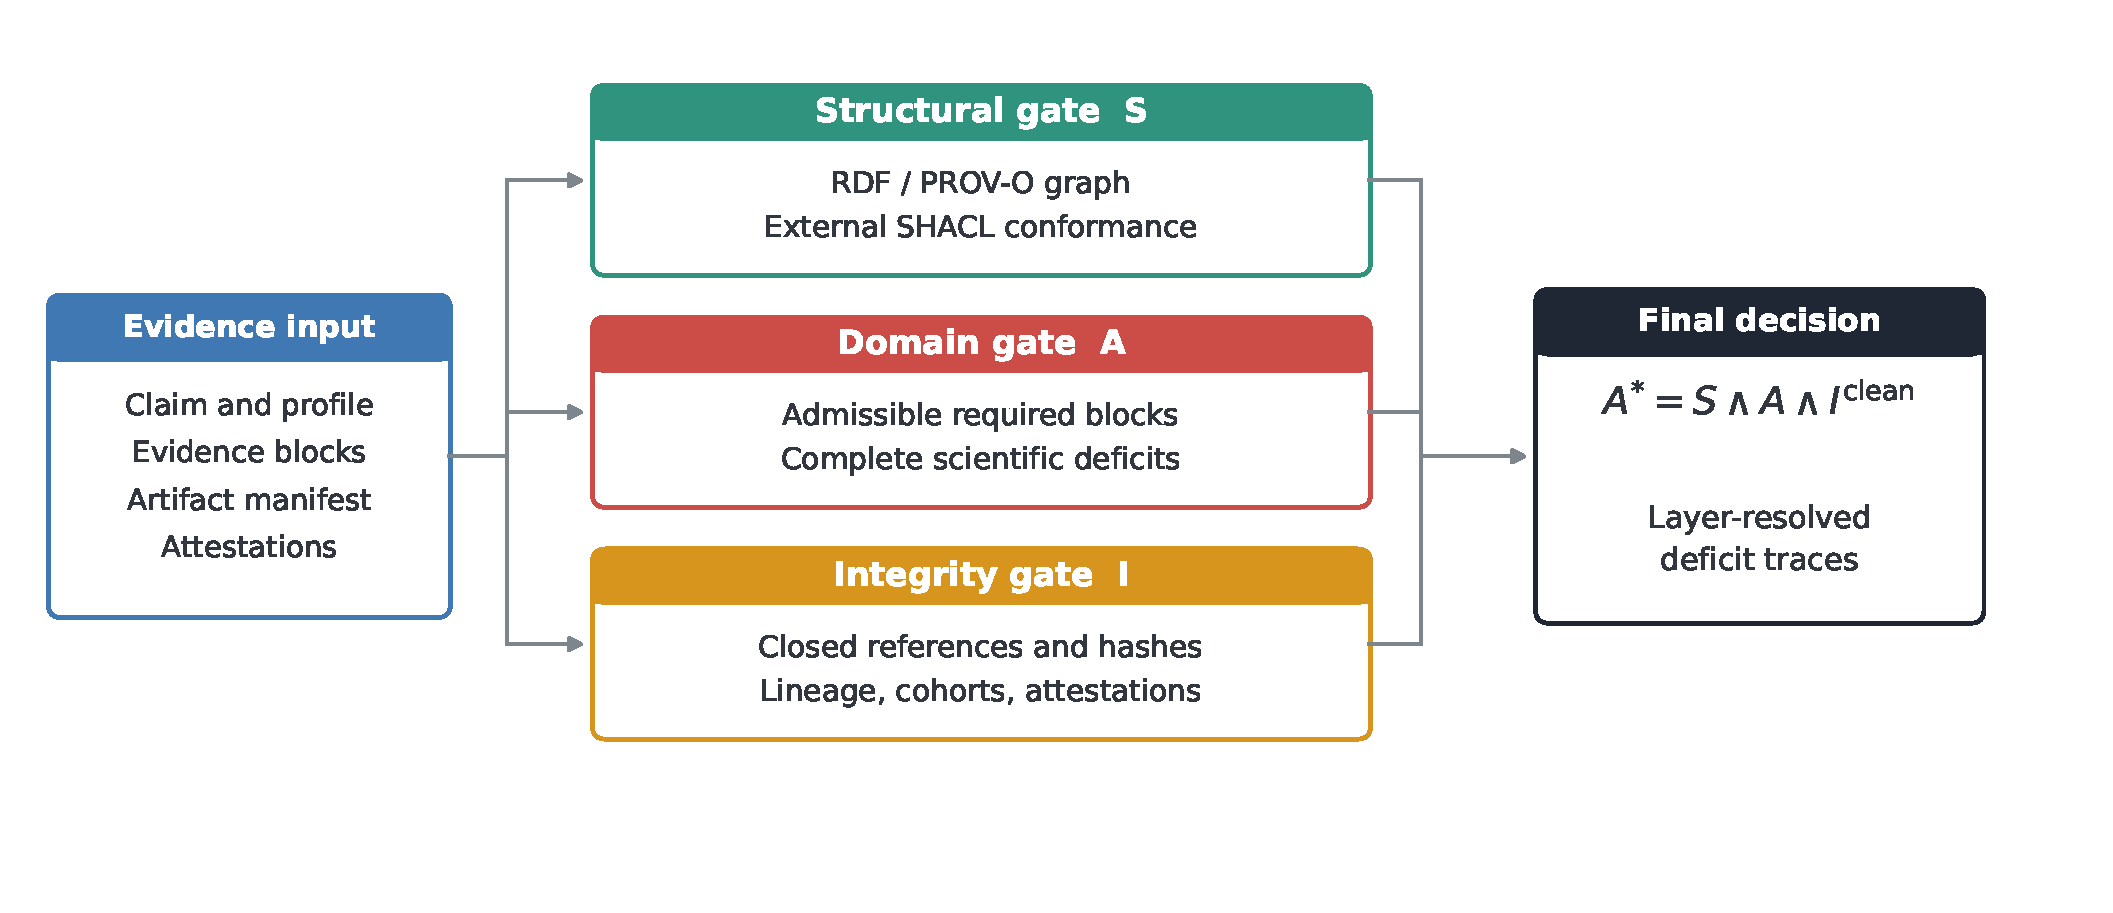
\includegraphics[width=0.98\textwidth]{Fig1.pdf}
\caption{Three-gate MouseClaimBench workflow. The same claim, evidence blocks, and manifest determine the RDF/PROV-O representation and enter structural conformance $S$, domain authorization $A$, and integrity analysis $I$. Only the empty-set predicate $I^{\mathrm{clean}}$ enters the Boolean composition $A^{*}=S\land A\land I^{\mathrm{clean}}$. A failure at any gate prevents authorization, while the output preserves every violated structural, scientific, and integrity category with an actionable witness}
\label{fig:standards-workflow}
\end{figure}

%% END ORIGINAL SOURCE: standards_workflow.tex




\subsection{Knowledge profile, evidence semantics, and symbolic authorization}
\label{subsec:authorization-semantics}

The domain knowledge used for authorization is represented through a
versioned profile

\begin{equation}
\Pi=\langle C,E,Q,O,V,H\rangle,
\label{eq:profile-v2}
\end{equation}

where $C$ is the claim vocabulary, $E$ is the evidence-block vocabulary,
$Q(c)\subseteq E$ is the set of mandatory blocks associated with claim $c$,
$O(e)$ is the set of observations required when block $e$ declares a pass,
$V$ is the profile version, and $H$ is its SHA-256 content identity.

The evaluated profile contains 10 claim types, 22 evidence-block types, and
60 claim--evidence requirements. Table~\ref{tab:profile-v2-claims}
enumerates the claim types, while
Fig.~\ref{fig:claim-evidence-matrix-v2} shows every required relation.
Authorization is evaluated independently for each claim from its own
required-block set $Q(c)$. The complete entity-specific mouse-brain
digital-twin claim (C10) requires 21 evidence blocks. Although some of these
blocks are also required by other claims, authorization of C1--C9 does not
combine or propagate to C10; C10 is authorized only when all evidence blocks
in $Q(\mathrm{C10})$ are admissible.



%% BEGIN ORIGINAL SOURCE: profile_v2_claims.tex (SHA256 506ba70ffcf2433e0acfb464eca0bc5653047ccb2a552cc2b08106471c1ee460)
\begin{table}[!htbp]
\centering
\caption{The 10 exact claim types in profile v2. Required-block counts sum to the 60 claim--evidence relations. Contract cases include independent source, rule, and rationale omissions and sum to 5,677}
\label{tab:profile-v2-claims}
\footnotesize
\renewcommand{\arraystretch}{1.08}
\begin{tabularx}{\textwidth}{@{}p{0.08\textwidth}Y r r@{}}
\toprule
Code & Claim type & Blocks & Cases \\
\midrule
C1 & Bounded predictive performance & 3 & 92 \\
C2 & Clean computational reproduction & 1 & 13 \\
C3 & Within-resource reproduction & 2 & 46 \\
C4 & Independent-study replication & 3 & 90 \\
C5 & Topology-specific prediction & 5 & 230 \\
C6 & Assumption-conditional direction & 4 & 150 \\
C7 & Local observational structure--function association & 6 & 321 \\
C8 & Intervention-supported effect & 5 & 228 \\
C9 & Directed topology-consistent prediction & 10 & 860 \\
C10 & Complete entity-specific mouse-brain digital twin & 21 & 3,647 \\
\midrule
Total & & 60 & 5,677 \\
\bottomrule
\end{tabularx}
\end{table}

%% END ORIGINAL SOURCE: profile_v2_claims.tex




%% BEGIN ORIGINAL SOURCE: claim_evidence_matrix_v2.tex (SHA256 d942d5d4e046c9870c80cba52c9f6488c819342ece26a3fb2457161604d38456)
\begin{figure}[!htbp]
  \centering
  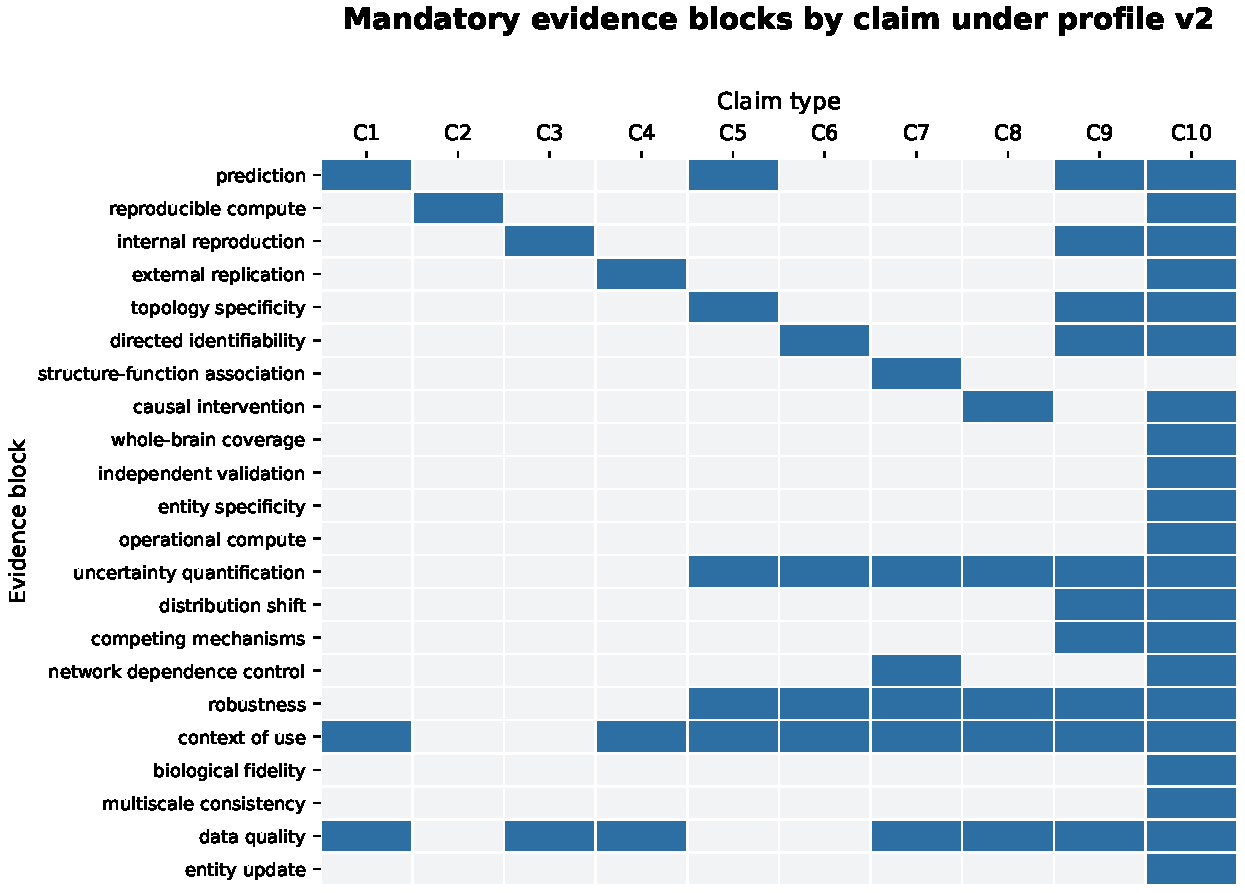
\includegraphics[width=0.92\textwidth]{Fig2.pdf}
  \caption{Complete profile-v2 claim--evidence matrix. Columns C1--C10 follow Table~\ref{tab:profile-v2-claims}, and rows correspond to the 22 evidence-block types. A filled cell indicates that the evidence block in that row is mandatory for the claim in that column under profile v2. The matrix contains 60 mandatory claim--evidence requirements in total; C10 has 21 required evidence blocks}
  \label{fig:claim-evidence-matrix-v2}
\end{figure}
%% END ORIGINAL SOURCE: claim_evidence_matrix_v2.tex



The profile is an explicit machine-readable knowledge specification rather
than a policy inferred from the conformance benchmark. Its acquisition
procedure first defines bounded claim wording and prohibited claim
promotions, then identifies distinct evidence functions from methodological
and mouse-brain sources, records their scope and exceptions, incorporates
findings identified through an internal adversarial audit, and verifies
executable and bibliographic coverage. The machine-readable basis contains
one stable record and one claim-specific necessity rationale for each of the
60 claim--evidence relations. Each relation is explicitly marked as a
source-grounded author requirement that has not been independently validated.
The cited sources justify the methodological role assigned to individual
evidence blocks; they are not represented as having prescribed the complete
authorization profile.

A separate, non-gating external content-validity protocol adapts established
procedures \citep{lynn1986content,terwee2018cosmin}. It specifies at least
seven independent experts, at least five years of relevant experience,
representation of three expertise strata, complete 1--4 ratings, item- and
scale-level content-validity indices, binary Fleiss agreement, and resolution
of every critical veto. Its acceptance thresholds were frozen before
recruitment. This protocol is not part of structural conformance $S_{\Pi}$,
domain authorization $A_{\Pi}$, or integrity conformance
$I^{\mathrm{clean}}_{\Pi}$ and does not affect any authorization decision
reported in this work.

The reasoning architecture also separates predicate execution from
authorization inference. Each of the 22 predicate contracts records whether
an upstream source adapter, a release adapter, or the authorization adapter
evaluates the corresponding scientific or operational rule. Together, the
contracts define 124 required observation slots. The responsible adapter
evaluates the predicate and preserves its rule, rationale, observations, and
artifact identity. The authorization engine then consumes these attested
predicate records, verifies the fields and observations required by the
profile, and applies $Q(c)$. It does not reduce prediction, topology,
intervention, anatomical coverage, reproducibility, and other heterogeneous
scientific quantities to a common numerical score.

An evidence block is represented as

\begin{equation}
b_e=\langle e,a,x,s,\phi,r\rangle,
\label{eq:evidence-block-v2}
\end{equation}

where $e\in E$ identifies the evidence-block type,
$a\in\{P,F,U,N,J\}$ denotes passed, failed, unknown, not targeted, or
requires review, $x$ contains the original-scale observations, $s$ identifies
the source artifact, $\phi$ is the predicate executed by the declared
evaluation adapter, and $r$ is its rationale. The authorization engine
therefore reasons over attested predicate records rather than recomputing
every source analysis. It also preserves observations in their original
scientific scale instead of normalizing correlation, matched-pair
differences, software revisions, interventions, and anatomical coverage into
a shared metric.

Let

\begin{equation}
\operatorname{present}(z)=
\begin{cases}
1, & \begin{aligned}[t]z\text{ is provided and is not an empty textual}\\\text{or container value}\end{aligned},\\
0, & \text{otherwise}.
\end{cases}
\label{eq:field-presence}
\end{equation}

Thus, valid numerical values such as zero count as present. A declared pass
is admissible only when the evidence block also contains its mandatory source,
predicate, rationale, and observation fields:

\begin{equation}
\operatorname{adm}_{\Pi}(b_e)=
\mathrm{1}[a=P]\operatorname{present}(s)\operatorname{present}(\phi)
\operatorname{present}(r)
\prod_{o\in O(e)}\operatorname{present}(x_o).
\label{eq:admissibility}
\end{equation}

Here, $\mathrm{1}[\cdot]$ is the indicator function. Consequently, blocks
with declared status $F$, $U$, $N$, or $J$ are non-admissible. A declared
pass is also non-admissible when its source, predicate, rationale, or a
required observation is absent. The admissibility rule prevents an upstream
source from asserting \emph{passed} while omitting observations required by
the profile, such as the target, split, comparator, inferential unit,
uncertainty method, or another contract-specific field.

For $c\in C$, the scientific deficit set is

\begin{equation}
\Delta_{\Pi}(c,B)=
\{e\in Q(c):\operatorname{adm}_{\Pi}(b_e)=0\},
\label{eq:scientific-deficits}
\end{equation}

where a required block absent from $B$ is materialized with unknown status.
The core symbolic authorization rule is non-compensatory:

\begin{equation}
A_{\Pi}(c,B)=
\begin{cases}
\mathrm{1}[\Delta_{\Pi}(c,B)=\varnothing], & c\in C,\\
0, & c\notin C.
\end{cases}
\label{eq:core-authorization}
\end{equation}

Authorization therefore requires every mandatory evidence block associated
with $c$ to be admissible. Evidence satisfying one requirement cannot
compensate for a deficit in another. The explicit outside-profile branch also
defines system behavior for claims not represented in $C$ without requiring
$Q(c)$ or $\Delta_{\Pi}(c,B)$ to be evaluated.

The same deficit semantics provide the explanation associated with a refusal.
For every member of $\Delta_{\Pi}$, the engine preserves the declared and
effective states, source, predicate, rationale, observations, and missing
fields. It does not reduce multiple failures to one prioritized explanation or
to a paper-level score. Category-complete reporting instead retains every
violated contract dimension together with an actionable witness. Completeness
is defined at the deficit-category level and does not require exhaustive
enumeration of redundant witnesses or every distinct cycle representing the
same violation category.

The fidelity of these explanations can be expressed counterfactually. Let
$T_R(B)$ replace exactly the evidence-block records indexed by a repair set
$R$ with complete admissible passing versions. A reported deficit set is
counterfactually sufficient and individually necessary when

\begin{equation}
A_{\Pi}(c,T_{\Delta_{\Pi}(c,B)}(B))=1
\quad\land\quad
\forall e\in\Delta_{\Pi}(c,B),\quad
A_{\Pi}(c,T_{\Delta_{\Pi}(c,B)\setminus\{e\}}(B))=0.
\label{eq:counterfactual-explanation}
\end{equation}

The first condition requires repairing every reported deficit to restore
authorization. The second requires authorization to fail again when any one
of those repaired deficits is individually restored. These properties evaluate
the fidelity of the explanation to the declared non-compensatory reasoning
model; they do not establish how useful a human reviewer finds the
explanation.


\subsection{Structural representation, provenance, and integrity reasoning}
\label{subsec:standards-integrity}

The knowledge profile and evidence package are exported as \ac{rdf} using
\ac{prov}. Profiles, claims, evidence blocks, artifacts, activities, and
authorization decisions receive stable identifiers. Artifact derivation uses
PROV relations, while profile-specific predicates represent mandatory
evidence and authorization state. The same graph can be serialized as Turtle
or JSON-LD. This representation provides interoperable exchange and
inspection while leaving scientific authorization to the executable reasoning
profile.

For each profile, MouseClaimBench generates \ac{shacl} shapes requiring the
package and profile identity, all mandatory block records, a status from the
allowed vocabulary, source, rule, rationale, and the observations required
when a block declares a pass. A third-party \texttt{pySHACL} processor
validates the resulting graph and returns structural deficits.

Structural conformance is deliberately distinct from scientific
admissibility. The shapes do not require an evidence block to have
\texttt{passed} status. A complete block with \texttt{failed} status is
therefore structurally conformant but scientifically non-admissible, allowing

\[
S_{\Pi}=1
\qquad\text{and}\qquad
A_{\Pi}=0
\]

for the same evidence package. \ac{shacl} consequently acts as an external
structural reasoning path rather than as a scientific authorization
mechanism.

In the current implementation, the structural contract applies to graphs
emitted by the MouseClaimBench serializer from typed evidence-package
objects. Arbitrary hostile third-party \ac{rdf} graphs fall outside this
contract; additional uniqueness constraints would be required to handle
duplicated or contradictory singleton values introduced directly into such
graphs.

The integrity reasoning layer evaluates relational conditions that cannot be
reduced to the presence of individual fields. Let $M$ contain the profile
identity, content-addressed artifact records, derivation edges,
block-to-artifact lineage, evidence attestations, and declared independence
relations. Its integrity deficit set $I_{\Pi}(M,B)$ records violations of the
13 conditions summarized in Table~\ref{tab:integrity-threat-model}.

Artifact identifiers and block-lineage declarations must be unique. All
artifact references from derivations, block lineage, attestations,
independence pairs, and disjoint-cohort pairs must resolve. Block lineage and
attestations must reference supplied evidence blocks. Every supplied block
requires lineage and at least one attestation, while each direct attestation
must agree with the represented block status. Independence and
cohort-disjointness relations must be irreflexive. The integrity taxonomy also
protects profile identity, artifact content, derivation order, and declared
independence. These conditions reflect established concerns in secure
provenance, assurance cases, and the avoidance of pseudoreplication
\citep{hasan2009provenance,mohamad2021assurance,lazic2010pseudoreplication}.



%% BEGIN ORIGINAL SOURCE: integrity_threat_model.tex (SHA256 d11e63ad7118ad9d5f488c8c0fe5d66f38717604260e56474275975ab317d0ce)
\begin{table}[!htbp]
\centering
\caption{Thirteen-type integrity model and evaluated coverage. O: 370-case original benchmark. C: 2,550-package compositional stress test. E: 100-package extended regression suite. D: six direct API edge-case regressions. O and C use the same eight historical attack families. The 20 trust-boundary controls are separate. These tests do not estimate attack prevalence or adaptive robustness}
\label{tab:integrity-threat-model}
\scriptsize
\renewcommand{\arraystretch}{1.06}
\begin{tabularx}{\textwidth}{@{}P{0.24\textwidth}P{0.16\textwidth}P{0.11\textwidth}Y@{}}
\toprule
Integrity condition & Protected asset & Evaluation & Violated invariant \\
\midrule
Profile-version substitution & Authorization contract & O, C & Identifier, version, and profile hash must match \\
Duplicate artifact identifier & Package namespace & D & Every artifact identifier must be unique within a package \\
Duplicate block lineage & Evidence trace & D & Every block must have one consolidated lineage declaration \\
Artifact-hash tampering & Source content & O, C & Declared and observed content identities must agree \\
Dangling provenance reference & Derivation graph & O, C, E & Every referenced artifact must resolve \\
Circular provenance & Derivation graph & O, C & Artifact derivation must be acyclic \\
Duplicate independent artifact & Independence declaration & O, C, D & Independence pairs must be irreflexive and cannot share content or composite generation identity \\
Overlapping independent cohorts & Inferential units & O, C, D & Cohort-disjointness pairs must be irreflexive and cannot share subjects \\
Contradictory attestation & Evidence status & O, C & One block cannot have incompatible source attestations \\
Missing block lineage & Evidence trace & O, C & Every supplied block must resolve to at least one source artifact \\
Unknown block reference & Evidence trace & E & Lineage and attestations must reference supplied blocks \\
Block--attestation mismatch & Evidence status & O, C, E & Every direct attestation must agree with the represented block status \\
Missing block attestation & Evidence trace & E & Every supplied block must have at least one source attestation \\
\bottomrule
\end{tabularx}
\end{table}

%% END ORIGINAL SOURCE: integrity_threat_model.tex



The cycle check uses an iterative depth-first traversal. Independence is
evaluated from content identity and from the composite identity
$(\texttt{study\_id},\texttt{data\_generation\_id})$ when both fields are
non-empty. The implementation does not assume that
\texttt{data\_generation\_id} is globally unique.

Duplicate identifiers remain invalid, but validation groups every declaration
instead of collapsing them. Reference closure considers all declarations,
cycle detection uses the union of their derivation edges, independence checks
evaluate all compatible record pairs, and cohort checks use the union
declared for each identifier. Input order therefore cannot hide a second
integrity-deficit category. These checks establish internal relational
consistency rather than external source trust or scientific independence.
Profile identity is checked at both the structural graph and manifest
boundaries, providing explicit defense in depth.

Because $I_{\Pi}(M,B)$ denotes a set of integrity deficits, its Boolean
conformance predicate is defined separately:

\begin{equation}
I^{\mathrm{clean}}_{\Pi}(M,B)=
\mathrm{1}[I_{\Pi}(M,B)=\varnothing].
\label{eq:integrity-clean}
\end{equation}

Structural conformance remains an independently executed reasoning path. The
graph is deterministically derived from the same claim, evidence blocks, and
manifest evaluated by the other layers:

\begin{equation}
G_{\Pi}(c,B,M)=\operatorname{RDF}_{\Pi}(c,B,M).
\label{eq:package-rdf}
\end{equation}

Let $S_{\Pi}(G)=1$ exactly when external \ac{shacl} validation reports no
structural violation against the shapes generated from $\Pi$. The field checks
in $S_{\Pi}$ intentionally overlap with defensive admissibility checks in the
Python core, but $S_{\Pi}$ is not absorbed into $A_{\Pi}$.

The final intelligent-system decision combines the three non-compensatory
reasoning dimensions:

\begin{equation}
A^{*}_{\Pi}(c,B,M)=
S_{\Pi}(G_{\Pi}(c,B,M))
\land A_{\Pi}(c,B)
\land I^{\mathrm{clean}}_{\Pi}(M,B).
\label{eq:integrity-authorization}
\end{equation}

Failure at any dimension prevents final authorization; no successful
dimension can compensate for another. A dedicated final authorization object
executes this composition while preserving separate structural, domain, and
integrity traces. Every reported deficit retains its corresponding witness.


\subsection{Multi-path reasoning, property verification, and release control}
\label{subsec:execution-release}

MouseClaimBench uses three deliberately scoped execution paths to evaluate
the authorization and conformance semantics: a primary Python reasoning path,
external \ac{shacl} structural validation, and a separately implemented
\ac{asp} reasoning path. Source-specific adapters provide the attested
predicate records consumed by these components, while a separate Python
integrity module evaluates relational package constraints.

The primary Python engine evaluates field presence, observation admissibility,
claim-specific domain requirements, and detailed scientific deficit
explanations. The external \ac{shacl} path evaluates only the structural
contract encoded in the \ac{rdf} graph. The separately implemented \ac{asp}
program receives declared statuses, metadata-presence facts, and
observation-presence facts and derives effective states, authorization, and
deficits within the Clingo ASP solver for every generated domain-contract
case.

Relational package integrity is evaluated before the three gate results are
composed. The Python and \ac{asp} paths share the profile specification but
not the inference implementation, while \ac{shacl} evaluates an externally
serialized structural representation. Agreement between Python and
\ac{asp}, together with conformance of the external \ac{shacl} results to the
structural expectations, therefore provides evidence about implementation
consistency within the declared reasoning semantics. It does not by itself
validate the scientific content of the shared profile.

The domain-reasoning property contract contains six package-level properties
of $A_{\Pi}$, with outside-profile closure evaluated separately as a boundary
condition. Soundness requires every domain-authorized claim to contain all
required admissible blocks. Completeness requires every package containing
all required admissible blocks to be domain-authorized. Deficit identity
requires the reported deficit set to equal the set defined in
Eq.~\ref{eq:scientific-deficits}.

Monotonic degradation requires replacing a passed evidence block with a
failed block to preserve or enlarge the deficit set and never create
authorization. Two additional properties require domain decisions to remain
invariant to evidence input order and to irrelevant unprofiled blocks.
Outside-profile closure requires every claim outside $C$ to remain outside
the authorization boundary.

Irrelevant-evidence invariance applies to the domain decision rather than to
arbitrary modifications of the final evidence package. Every supplied block
must still satisfy manifest lineage and attestation requirements, even when it
is irrelevant to $Q(c)$. These properties are evaluated over generated
packages and characterize the implemented reasoning contract; they are not
an exhaustive proof over arbitrary future profiles.

Release control provides a final reproducibility layer around the executable
system. Release artifacts record protocol hashes, profile hashes, source
revisions, exact public asset identifiers, and official data hashes. A release
is rejected when a required artifact is absent, any source revision ends in
\texttt{-dirty}, an expected benchmark decision changes, or a broad
prohibited claim becomes true. These checks enforce reproducibility and scope
preservation without changing the structural, domain, or integrity semantics
defined above. They do not establish external source trust or independent
scientific consensus on the authorization profile.
%% END ORIGINAL SOURCE: method.tex



%% BEGIN ORIGINAL SOURCE: experiments.tex (SHA256 b33fab42b84e574b9ba41bf53f0dc219c1237fe46f2e23cbfa8b92f12247c2ac)
\noindent\textbf{Editorial preparation and author oversight.}
Following completion of the reported experiments, an AI assistant was used to consolidate the manuscript's LaTeX files and propose journal-specific editorial wording. This assistance did not produce new study data, experiments, or numerical outcomes. Scientific claims, interpretation, and final wording remain the responsibility of the human authors.

\section{Experimental Evaluation of Knowledge-Based Authorization}
\label{sec:experiments}
The evaluation examines MouseClaimBench from five complementary perspectives: knowledge-profile traceability, reasoning conformance and explanation fidelity, integrity robustness, computational performance, and artifact-grounded scientific application. These perspectives are kept separate because they support different conclusions. Conformance experiments test whether the implemented reasoning follows the declared authorization semantics; counterfactual experiments test whether reported deficits faithfully explain refusal; integrity experiments characterize resistance to declared package violations and expose the trust boundary; performance experiments characterize the cost of the implemented reasoning components; and artifact-grounded applications evaluate the decisions produced when the same frozen authorization semantics are applied to public computational neuroscience resources.

The evaluation does not use software conformance as evidence that the scientific content of the profile is universally valid. Likewise, empirical authorization under the profile is not interpreted as biological truth. Table~\ref{tab:experiment-design-v2} summarizes the evaluation questions, evidence units, and supported interpretations associated with each experiment.



%% BEGIN ORIGINAL SOURCE: experiment_design_v2.tex (SHA256 47ad8da81b7c784577eaf63419548113c7cf58a2872c4c766261481ff086613c)
\begin{table}[!htbp]
\centering
\caption{Evaluation questions, evidence units, and supported interpretations}
\label{tab:experiment-design-v2}
\scriptsize
\setlength{\tabcolsep}{3pt}
\renewcommand{\arraystretch}{0.95}

\begin{tabularx}{\textwidth}{
@{}
P{0.05\textwidth}
P{0.25\textwidth}
P{0.31\textwidth}
Y
@{}}
\toprule
ID &
Evaluation question &
Evidence unit &
Supported interpretation \\
\midrule

K1 &
Is the knowledge profile fully traceable?
&
10 claims, 22 predicates, 60 relations, 124 observation slots
&
Traceability of the author-defined profile
\\

V1 &
Does reasoning conform to the declared semantics?
&
5,677 Python/\ac{asp} cases, 5,677 \ac{shacl} cases, 8 gate states, 10,000 generated packages
&
Domain, structural, and compositional conformance
\\

V2 &
Are decisions monotonic and explanations faithful?
&
221 profile variants, 10,000 counterfactual packages, 60 single-relation degradations
&
Local sensitivity, sufficiency, necessity, and deficit retention
\\

T1 &
Does integrity reasoning enforce declared invariants?
&
370 original cases, 2,550 attack compositions, 100 regressions, 6 API cases, 8 ablations, 20 forgery controls
&
Robustness to declared violations and explicit trust boundary
\\

P1 &
What is the computational cost of authorization?
&
Up to 10,000 packages and 5,000 artifacts
&
Component-level performance on one host
\\

A1 &
Are bounded interpretations preserved on real artifacts?
&
5 retrospective targets, 5 strict twin claims, and \ac{microns}
&
Profile-relative authorization without claim promotion
\\

A2 &
Can frozen rules preserve unseen positive and negative outcomes?
&
2 \ac{dandi} resources with pre-access protocols
&
Prospective authorization and refusal under fixed rules
\\

\bottomrule
\end{tabularx}
\end{table}
%% END ORIGINAL SOURCE: experiment_design_v2.tex




\subsection{Evaluation design and decision rules}
\label{subsec:experimental-design}
The first evaluation component audits whether the executable knowledge profile is traceable to its machine-readable acquisition record and bibliographic basis. Acceptance requires exact coverage of the 10 claim definitions, 22 evidence-block types, 22 predicate contracts, and 60 claim--evidence relations. Every relation must have a unique identifier and a claim-specific necessity rationale. Every predicate contract must specify evaluation ownership, decision-rule scope, required observations, sources, and exceptions. All source identifiers must resolve to the bibliography. Independent content validity and human validation remain explicitly recorded as unavailable rather than being inferred from implementation conformance.

The historical 29-item v1 review instrument is excluded from the evaluation. A separate v2 protocol contains 92 prospective review items covering the 10 claims, 22 predicates, and 60 relations. It requires at least seven eligible independent experts and predefined conditions for item-level content validity, scale-level content validity, agreement, and critical vetoes. At the time of the present evaluation, the protocol has no completed eligible independent raters and therefore contributes no evidence to the reported results.

The reasoning-conformance benchmark generates eight case families from every profile claim. These families comprise a pristine complete package, single-block mutations to each of the four non-passing states, omission of one mandatory block, omission of one required observation, separate omission of source, rule, or rationale, and all $16$ combinations of non-passing states for each pair of required blocks.

For a claim with $q_c$ required blocks and $m_c$ mandatory observation fields across those blocks, the number of generated cases is

\begin{equation}
N_c=1+8q_c+m_c+16\binom{q_c}{2}.
\label{eq:contract-case-count}
\end{equation}

The constant term counts the single pristine package. The coefficient $8q_c=(4+1+3)q_c$ counts, for each required block, four single-block mutations to the non-passing states, one block omission, and three independent metadata omissions corresponding to source, rule, and rationale. The term $m_c$ counts one omission for each mandatory observation field. Finally, $16\binom{q_c}{2}$ counts the $4\times4$ combinations of non-passing states for every unordered pair of required blocks.

Table~\ref{tab:profile-v2-claims} reports every $N_c$, which sums to $5,677$. Each case has an exact expected domain-authorization decision and deficit set derived from Eqs.~\ref{eq:admissibility}--\ref{eq:core-authorization}. The primary Python reasoning engine and the separately implemented \ac{asp} program evaluate all $5,677$ domain cases. External \ac{shacl} validation evaluates structural conformance and structural deficits over the same packages. Non-passing statuses remain structurally valid, whereas block, metadata, and required-observation omissions are structural failures. JSON-LD round-trip equivalence is evaluated through graph isomorphism. A separate truth-table benchmark evaluates all eight combinations of $S_{\Pi}$, $A_{\Pi}$, and integrity conformance against Eq.~\ref{eq:integrity-authorization}.

Property-based verification evaluates the operational semantics of $A_{\Pi}$ on $1,000$ deterministically generated random evidence packages for each of the 10 claims. Every package is tested for soundness, completeness, exact deficit identity, input-order invariance, irrelevant-evidence invariance, and monotonic degradation whenever a passed block exists. Outside-profile closure is evaluated separately. Property-based tests also generate additional status and observation mutations during the software test suite. The reported $55,031$ checks correspond to the frozen deterministic experiment over $A_{\Pi}$ rather than to an exhaustive proof over arbitrary future profiles or the complete package-integrity semantics.

A separate one-edge policy-perturbation experiment evaluates the local sensitivity of authorization decisions to changes in the claim--evidence profile. Fourteen claim--package instances are held fixed: the bounded target claim and strict complete-twin claim for each of five retrospective cases and two pre-access \ac{dandi} cases. The experiment evaluates the baseline profile, all 60 profiles obtained by removing one required relation, and all 160 profiles obtained by adding one currently unrequired evidence block to one claim. Let $x_j=(c_j,B_j)$ denote one fixed claim and evidence package. For profile variant $\Pi_k$, the decision-flip indicator is

\begin{equation}
F_{jk}=\mathrm{1}\!\left[
A_{\Pi_k}(c_j,B_j)\neq A_{\Pi}(c_j,B_j)
\right].
\label{eq:profile-sensitivity-flip}
\end{equation}

Core domain authorization is used deliberately in this experiment to isolate the scientific relation policy while manifests remain pristine and graphs remain structurally conformant. Removing one relation weakens the profile and can only expand authorization. Adding one relation strengthens the profile and can only contract authorization when the added block is not admissibly passed. Decision flips therefore provide expected monotonicity probes under local profile changes. They identify decisive relations for the fixed packages; they do not establish that an alternative profile is scientifically preferable.

Explanation fidelity is evaluated independently on a deterministic set of $1,000$ packages per claim. Every non-authorized package is repaired by replacing exactly the reported deficits with complete passing attestations. Counterfactual sufficiency requires the repaired package to authorize with no residual deficit. Individual necessity is then tested by restoring each repaired block in turn to its original defective state; authorization must again fail with that block as the sole remaining deficit, implementing Eq.~\ref{eq:counterfactual-explanation}. Every witness must retain a non-empty block name, source, rule, and rationale.

Finally, each of the 60 pristine claim--evidence relations is degraded independently. A single-reason explanation baseline is evaluated descriptively by counting how many simultaneous deficits it would omit. This experiment assesses information retention and counterfactual fidelity of the symbolic explanation mechanism; it does not test perceived usefulness to human reviewers.

The integrity evaluation uses a controlled threat model derived from the conditions in Table~\ref{tab:integrity-threat-model}. The original benchmark contains 370 cases. For each of the 10 claims, it includes one pristine package, every individual attack from the eight historical attack families, and all 28 pairwise attack combinations, producing 360 attacked packages.

The structural gate is excluded from this benchmark to isolate the behavior of package-integrity controls, including manifest-level profile identity. For integrity configuration $k$, $I^{\mathrm{clean}}_{\Pi,k}$ denotes integrity conformance under the controls retained by configuration $k$, following Eq.~\ref{eq:integrity-clean}. The domain-plus-integrity decision is

\begin{equation}
A^{I}_{\Pi,k}(c,B,M)=
A_{\Pi}(c,B)
I^{\mathrm{clean}}_{\Pi,k}(M,B).
\label{eq:integrity-ablation-decision}
\end{equation}

Let $\mathcal{D}_{\mathrm{attack}}$ denote the benchmark cases, with claim $c_z$, evidence blocks $B_z$, and manifest $M_z$ for case $z$. The configuration-specific false-authorization rate over the controlled attack benchmark is:

\begin{equation}
\operatorname{FAR}^{(k)}_{\mathrm{attack}}=
\frac{
\sum_{z\in\mathcal{D}_{\mathrm{attack}}}
\mathrm{1}[z\text{ attacked}]
A^{I}_{\Pi,k}(c_z,B_z,M_z)
}{
\sum_{z\in\mathcal{D}_{\mathrm{attack}}}
\mathrm{1}[z\text{ attacked}]
}.
\label{eq:attack-far}
\end{equation}

The complete domain-plus-integrity configuration is compared with the domain-only profile, a hash-only baseline, and eight leave-one-control-out configurations. Exact trace recovery requires the detected deficit codes to equal every invariant violated by the applied attacks. Full $S_{\Pi}\land A_{\Pi}\land I^{\mathrm{clean}}_{\Pi}$ composition is evaluated separately through the eight-state truth table. The ablation comparison therefore evaluates integrity configurations rather than replacing evaluation of the final authorization object.

The compositional stress test evaluates all $2^8-1=255$ non-empty subsets of the eight historical attack families for each claim, yielding 2,550 attacked packages. A separate nine-family extended regression suite contains 10 pristine and 90 reference- or attestation-level cases. Six direct API cases cover duplicate identifiers, reflexive relations, and both branches of study-scoped data generation identity. Twenty trust-boundary controls alter content and hashes coherently or forge internally consistent independence metadata. These controls are expected to remain authorized when no externally verifiable contradiction is available, thereby exposing the boundary between internal integrity reasoning and external source authentication.

Computational performance is evaluated separately from reasoning correctness. The core authorization-engine microbenchmark is executed on one Apple arm64 host with Python 3.12.13. Pristine authorization batches contain 100, 1,000, and 10,000 packages drawn cyclically from all profile claims. Each batch is repeated five times after 100 warm-up decisions. A separate timed component expands one valid digital-twin package to 25, 100, 1,000, and 5,000 uniquely content-addressed artifacts and evaluates the integrity layer.

Median wall-clock time and all repetitions are stored. Downloads, source-predicate execution, graph serialization, and external \ac{shacl} validation are excluded. These measurements therefore characterize component-level execution on one implementation and host rather than end-to-end system scalability or a portable latency guarantee.

Artifact-grounded evaluation complements the synthetic and controlled benchmarks. The first component reuses five frozen result packages assembled during the MouseBrainBench study
(\MouseBrainBenchCompanion) and asks whether profile v2 authorizes their bounded target claim and strict digital-twin claim. These mappings are retrospective authorization experiments and are not counted as prospective external validation.

The second component applies dependence-aware inference to \ac{microns}. The analysis specification and positive direction were fixed in the discovery window and subsequently evaluated in two non-overlapping hold-out windows within the same tissue volume. Directed-pair regression controls log soma
distance, its square, pre- and postsynaptic degree, and coarse cell type. Dependence is addressed through directed dyadic cluster covariance and 1,000 simultaneous node-label Freedman--Lane permutations. These hold-outs provide internal reproduction rather than independent biological replication.

The third component evaluates two external \ac{dandi} protocols frozen before numerical asset access.

For the \ac{microns} permutation test, the full model regresses readout-location similarity $y_{ij}$ on the directed connection indicator $c_{ij}$ and the fixed control vector $z_{ij}$:

\begin{equation}
y_{ij}=
\beta_0+\beta_1c_{ij}+z_{ij}^{\top}\gamma+\varepsilon_{ij}.
\label{eq:microns-full-model}
\end{equation}

The reduced model omits $c_{ij}$. Its residuals are placed in a directed neuron-by-neuron array. The connection indicator is residualized against the same controls, and the resulting residualized coefficient is used as the test statistic. Each permutation draws one permutation of neuron identifiers and applies it simultaneously to sender and receiver indices of the reduced-model residual array. This preserves reciprocal array structure and the incidence pattern induced by shared neurons under relabelling.

The discovery window fixes the positive direction and analysis specification. Its one-sided permutation value is reported descriptively and has no confirmatory interpretation. The dyadic regression is reported with a two-sided test and $95\%$ confidence interval in every window. The
confirmatory one-sided permutation test is subsequently evaluated in the two pre-fixed hold-outs. Its finite-permutation value is $(1+K)/(1+R)$, where $K$ is the number of permuted coefficients at least as large as the observed positive coefficient and $R=1000$.

Discovery and the two hold-outs use reproducible streams with seeds 2026080201, 2026080202, and 2026080203. A hold-out passes only when $\widehat{\beta}_1>0$, $p_{\mathrm{dyadic}}\leq0.05$, and
$p_{\mathrm{perm}}\leq0.05$. Confirmation requires this conjunction in both fixed hold-outs after a positive discovery direction. The procedure assumes exchangeability of the reduced-model residual array under simultaneous node relabelling.

Two external \ac{dandi} protocols were committed before numerical asset access. The availability protocol was frozen in commit \texttt{b59a497} and the predictive protocol in \texttt{d039e66}. Their SHA-256 identities are retained in the result artifact, and the numerical result was committed later.
This Git history provides temporal evidence for the declared ordering rather than third-party preregistration.

DANDI:001176 was selected from metadata describing 29 subjects and simultaneous cholinergic axon, cortical \ac{ach}, pupil, and treadmill signals \citep{neyhart2024ach}. The frozen protocol required at least 20 usable subjects and prohibited threshold or endpoint repair. After catalog inspection, the 28 schema-valid sessions represented only 5 subjects, so the predictive model was not executed.

DANDI:000039 contains contrast-tuning recordings associated with a published
visual-cortex study \citep{millman2020vip}. Before inspecting its asset
catalog or numerical values, the protocol fixed one lexicographically first
\texttt{behavior+ophys.nwb} asset per mouse, a trial-level population mean
event response, ridge regression with $\alpha=1$, and an intercept comparator.

For contrast $q$ and direction $\theta$ in degrees, the exact five regressors
are
$\log(1+100q)$,
$\sin(\theta)$,
$\cos(\theta)$,
$\log(1+100q)\sin(\theta)$, and
$\log(1+100q)\cos(\theta)$.
Angular functions are evaluated after conversion to radians.

The first 60\% of trials train the model, the next 20\% remain reserved, and
the final 20\% form the test partition. The intermediate partition is
deliberately unused. It does not affect model fitting, model selection,
threshold definition, or final evaluation. The \texttt{StandardScaler} is
fitted on the training partition only and then applied unchanged to the
held-out partition. Ridge $\alpha=1$ is fixed and no tuning occurs after
asset access.

The per-mouse held-out metric is Pearson correlation. Authorization requires
at least 25 usable mice, median held-out correlation of at least 0.10, a
positive 95\% mouse-bootstrap lower bound, at least 65\% of mice with
positive held-out correlation, and trial-pooled mean squared error below the
intercept. For $M$ mice with $n_m$ held-out trials,

\begin{equation}
\operatorname{MSE}_{\mathrm{pool}}=
\frac{
\sum_{m=1}^{M}
\sum_{t=1}^{n_m}
(y_{mt}-\widehat{y}_{mt})^2
}{
\sum_{m=1}^{M}n_m
}.
\label{eq:dandi-pooled-mse}
\end{equation}

The implementation stores and compares the two squared-error numerators
because their denominator is identical. The resulting metric weights mice in
proportion to their number of held-out trials. All authorization conditions
must pass.

The bootstrap uses protocol seed 2026080202 and resamples mice with
replacement 5,000 times. Each replicate computes the median mouse-level
Pearson correlation. The reported lower bound is its 2.5th percentile and
therefore targets population stability across mice rather than trial-level
independence.

These thresholds are author-defined operational acceptance criteria rather
than criterion-validated biological standards. The 25-mouse requirement
preserves a multi-mouse endpoint and supports a meaningful mouse-level
bootstrap but was not derived from a formal power calculation. The 0.10
median-correlation threshold requires a minimum predictive signal, the
positive bootstrap lower bound requires population-level sign stability, the
65\% rule requires a majority of mice to have positive held-out correlations
while tolerating heterogeneity, and the intercept comparison requires
incremental predictive value. The 20-subject availability boundary for
DANDI:001176 similarly protects the intended cross-subject design but is not
a general sufficiency standard.

A post-outcome sensitivity analysis changes one threshold at a time while
holding all other frozen conditions fixed. Its role is to expose decision
margins rather than to recalibrate or replace either protocol.


\subsection{Knowledge-profile traceability, sensitivity, and explanation fidelity}
\label{subsec:construct-validity-results}

The acquisition audit exactly covers the 10 claims, 22 evidence blocks, 22
predicate contracts, 60 claim--evidence relations, and 124 required
observation slots. All 60 relation identifiers and necessity rationales are
unique, and all 20 source identifiers resolve to the bibliography. The ledger
separates upstream predicate execution from authorization inference and marks
every relation as a source-grounded author requirement that has not been
independently validated.

These results establish complete traceability of the executable profile to its
declared knowledge-acquisition record. They do not establish that the profile
is scientifically complete, optimal, or universally accepted.

The one-edge analysis evaluates 221 profiles and 3,094 profile--case
combinations. The baseline authorizes four of the 14 fixed decisions. Among
the 60 weakening variants, only removal of the
\texttt{data\_quality} requirement from bounded prediction changes an
authorization. It converts the Dynamic Sensorium target from a documented
quality refusal into an authorization. This result identifies the requirement
that is decision-critical for that package rather than showing that the
requirement should be removed.

Among the 160 strengthening variants, 52 change at least one authorization
decision and produce 71 contractions. These contractions follow the expected
non-compensatory monotonicity of the system because an otherwise authorized
package lacks an admissible attestation for the newly introduced requirement.
Ninety-six variants change at least one deficit set even when the final
authorization decision remains unchanged. The perturbation counts therefore
characterize local decision sensitivity of the declared reasoning policy
rather than providing independent scientific evidence for alternative
claim--evidence relations. Table~\ref{tab:profile-sensitivity-v2} summarizes the local profile-perturbation results.



%% BEGIN ORIGINAL SOURCE: profile_sensitivity_v2.tex (SHA256 40d22e064e6c7d92f264d9c175e67e9f9452dd7a709e6e655d76d2df4bdb0e3d)
\begin{table}[!htbp]
\centering
\caption{One-edge structural policy perturbation across 14 fixed artifact decisions. Expansions are refusals authorized after removing one requirement. Contractions are authorizations withdrawn after adding one block. The monotonicity probe identifies decisive relations in these packages. The variants are not scientifically validated candidate profiles}
\label{tab:profile-sensitivity-v2}
\scriptsize
\renewcommand{\arraystretch}{1.00}
\begin{tabularx}{\textwidth}{@{}P{0.18\textwidth}rrrrY@{}}
\toprule
Policy set & Variants & Runs & With flips & Flips & Interpretation \\
\midrule
Baseline profile & 1 & 14 & -- & 0 & Four bounded authorizations \\
Remove one required relation & 60 & 840 & 1 & 1 expansion & Removing data quality authorizes the otherwise refused Dynamic Sensorium target \\
Add one unrequired block & 160 & 2,240 & 52 & 71 contractions & Positive cases lose authorization when the added block lacks an admissible attestation \\
\midrule
Total & 221 & 3,094 & 53 & 72 & One-at-a-time structural policy envelope \\
\bottomrule
\end{tabularx}
\end{table}

%% END ORIGINAL SOURCE: profile_sensitivity_v2.tex



Counterfactual explanation fidelity is evaluated on 10,000 packages. Of the
9,839 non-authorized packages, repairing every reported deficit satisfies
counterfactual sufficiency: every repaired package becomes authorized with no
residual deficit.

Restoring each repaired deficit individually produces 51,480
individual-necessity checks. Every check results in refusal, with the restored
deficit as the sole remaining deficit. The same 51,480 deficit records retain
non-empty witnesses, and all 60 pristine single-block degradations return the
expected sole deficit.

There are 8,632 packages containing simultaneous deficits. A single-reason
trace would retain only 9,839 deficits and would therefore omit

\[
51{,}480-9{,}839=41{,}641
\]

deficit records. This comparison quantifies information retained by the
category-complete symbolic explanation mechanism under the generated
packages. It does not measure human-perceived explanation quality.


\subsection{Reasoning conformance and property-based verification}
\label{subsec:conformance-results}

Table~\ref{tab:standards-formal-results} reports the multi-path reasoning and
conformance results. The primary Python engine produces no false
authorization or rejection across all 5,677 contract cases and recovers every
expected domain-deficit set. The separately implemented \ac{asp} reasoning
path matches all domain-authorization decisions and deficit sets while
deriving admissibility inside the Clingo solver.

External \ac{shacl} validation returns every expected structural decision and
deficit, including status-only domain failures that remain structurally valid
while scientifically unauthorized. The outcomes for all eight combinations
of structural, domain, and integrity conformance match
Eq.~\ref{eq:integrity-authorization}.

The exported 318-triple \ac{rdf} profile represents every claim and
evidence-block type. JSON-LD round trips preserve graph isomorphism in five
packages spanning pristine, scientific-failure, structural-failure,
rich-manifest, and digital-twin-style cases.



%% BEGIN ORIGINAL SOURCE: standards_formal_results.tex (SHA256 99f7b2f8438478c8e5730812f7bd72d05106d142f76a8d1e424f9bc28fa53ca2)
\begin{table}[!htbp]
\centering
\caption{Conformance and domain-gate property results. Exactness is relative to the frozen profile-v2 contract, and each engine is reported only for its evaluated comparison set}
\label{tab:standards-formal-results}
\footnotesize
\renewcommand{\arraystretch}{1.08}
\begin{tabularx}{\textwidth}{@{}p{0.26\textwidth}r r Y@{}}
\toprule
Evaluation & Cases/checks & Errors & Result \\
\midrule
Python contract mutations & 5,677 & 0 & Exact domain authorization and deficits \\
Independent \ac{asp} conformance & 5,677 & 0 & 100\% domain-status and deficit agreement \\
External \ac{shacl} conformance & 5,677 & 0 & Exact structural conformance and structural deficits \\
Three-gate composition & 8 states & 0 & Exact $S\land A\land I^{\mathrm{clean}}$ truth table \\
JSON-LD round trips & 5 graphs & 0 & Isomorphic \ac{rdf} graphs \\
Domain-gate property benchmark & 55,031 & 0 & Six core properties and outside closure hold \\
\bottomrule
\end{tabularx}
\end{table}

%% END ORIGINAL SOURCE: standards_formal_results.tex



The agreement between Python and \ac{asp} provides cross-implementation
evidence for the domain reasoning semantics. External \ac{shacl} validation
provides an independently executed structural path and deliberately neither
recomputes source predicates nor evaluates relational package integrity.
Together, these paths test the separation and composition of the proposed
reasoning architecture while remaining scoped to the declared authorization
profile.

The 10,000 deterministically generated random evidence packages yield 55,031
domain-reasoning property checks with no violation. Soundness, completeness,
deficit identity, input-order invariance, and irrelevant-evidence invariance
each pass 10,000 checks. Monotonic degradation passes all 5,030 applicable
checks. Outside-profile closure also passes.

These results support implementation conformance to the operational semantics
of $A_{\Pi}$ under profile v2. They do not prove scientific completeness of
the profile or behavior over every possible future profile.


\subsection{Integrity robustness, ablation, and computational performance}
\label{subsec:integrity-results}

Under the declared deterministic threat model, the complete
domain-plus-integrity configuration returns the expected integrity-deficit
trace in all 370 benchmark packages. It produces no false rejection on the 10
pristine packages and no false authorization on the 360 attacked packages.

The domain-only configuration does not reason over package integrity and
therefore authorizes all 360 attacked packages. Hash checking alone blocks
content tampering but authorizes 280 packages affected by profile
substitution, broken or cyclic lineage, false independence, cohort overlap,
contradictory attestations, or missing block provenance. The structural gate
is excluded from these counts so that manifest-level profile substitution
remains observable in the integrity experiment rather than being rejected
earlier by structural profile-identity matching. Fig.~\ref{fig:integrity-ablation-v2} illustrates the different false-authorization rates under those isolated configurations.



%% BEGIN ORIGINAL SOURCE: integrity_ablation_v2_figure.tex (SHA256 df53f94f48ee2feeeb072214d3c5147532b4132c52c4addc46ffe14db3777f93)
\begin{figure}[!htbp]
\centering
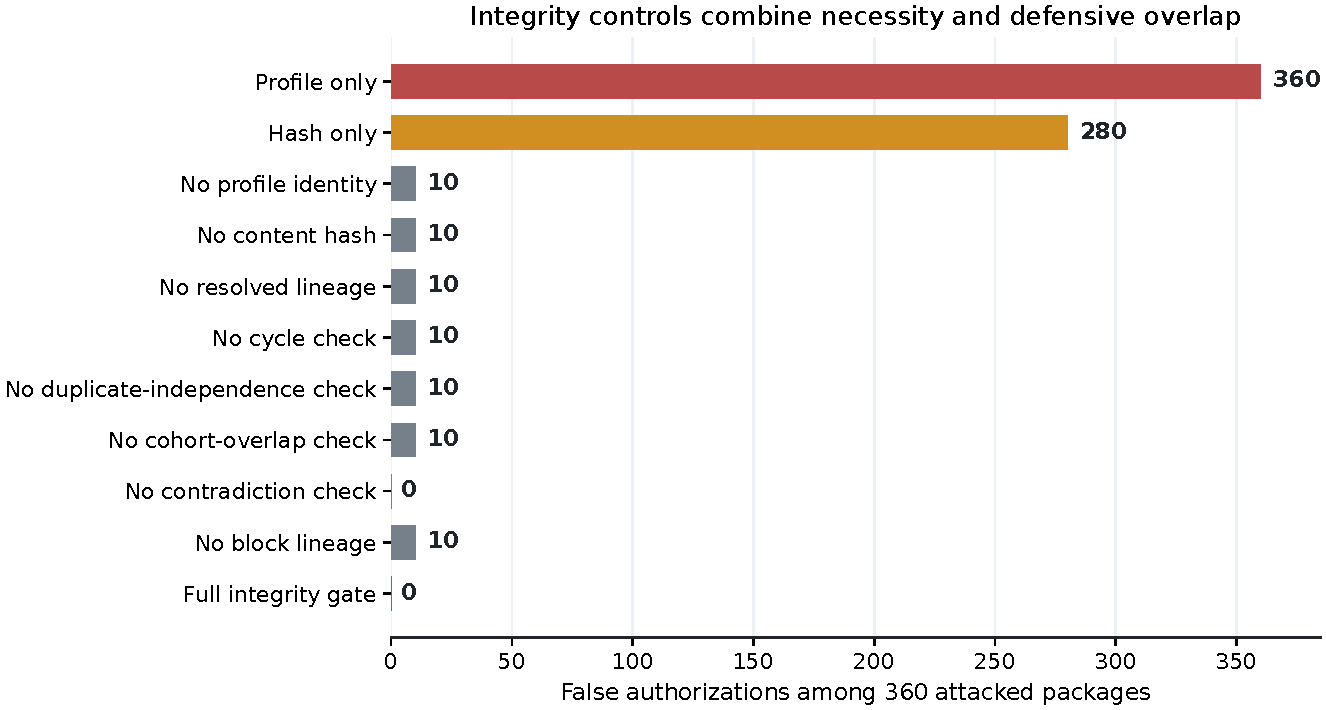
\includegraphics[width=0.96\textwidth]{Fig3.pdf}
\caption{False authorizations among 360 attacked packages across 10 profile claims, where lower values are better. The structural gate is excluded to isolate the domain-plus-integrity configurations. The profile-only baseline authorizes all 360 attacked packages. The hash-only baseline authorizes 280 packages involving identity, lineage, dependence, conflict, or provenance. The full integrity configuration blocks every declared attack. Seven original control omissions expose 10 packages each. Removing the contradiction check alone exposes none because block--attestation status consistency detects the same contradictory packages}
\label{fig:integrity-ablation-v2}
\end{figure}

%% END ORIGINAL SOURCE: integrity_ablation_v2_figure.tex



The leave-one-control-out experiment distinguishes unique necessity from
defensive overlap. Removing any of seven original controls creates 10 false
authorizations, corresponding to the single-attack package for that omitted
control in each claim. Removing only the contradictory-attestation check
creates no false authorization because the same packages also violate
block--attestation status consistency. Pairwise attacks containing another
enabled control remain blocked.

Table~\ref{tab:integrity-ablation-v2} reports the exact values, while
Fig.~\ref{fig:integrity-ablation-v2} visualizes the contrast between incomplete
baselines and the complete domain-plus-integrity architecture. The experiment
therefore identifies conditional necessity and one explicit instance of
defensive redundancy under the declared attack construction.



%% BEGIN ORIGINAL SOURCE: integrity_ablation_v2.tex (SHA256 493414ea72ced00ad730e1d337a780d7ff7b6dd52ad8f3838d6f572c92266b09)
\begin{table}[!htbp]
\centering
\caption{False authorizations and false rejections for domain-plus-integrity configurations in the 370-case integrity benchmark. The structural gate is excluded to isolate manifest-level controls. Seven original controls are uniquely necessary for their constructed single-attack families. Removing the contradiction check alone produces no false authorization because block--attestation status consistency independently detects the same contradictory package}
\label{tab:integrity-ablation-v2}
\footnotesize
\renewcommand{\arraystretch}{1.05}
\begin{tabularx}{\textwidth}{@{}Y r r@{}}
\toprule
Integrity configuration & False authorizations / 360 & False rejections / 10 \\
\midrule
Profile without integrity & 360 & 0 \\
Hash-only integrity & 280 & 0 \\
Full integrity gate & 0 & 0 \\
Without profile identity & 10 & 0 \\
Without content hash & 10 & 0 \\
Without resolved lineage & 10 & 0 \\
Without cycle detection & 10 & 0 \\
Without duplicate-independence check & 10 & 0 \\
Without cohort-overlap check & 10 & 0 \\
Without contradictory-attestation check & 0 & 0 \\
Without block lineage & 10 & 0 \\
\bottomrule
\end{tabularx}
\end{table}

%% END ORIGINAL SOURCE: integrity_ablation_v2.tex



The compositional stress test evaluates 2,560 packages: 10 pristine packages
and 2,550 attacked packages. For every claim, the attacked cases span all 255
non-empty compositions of the eight historical attack families. The complete
domain-plus-integrity configuration produces no false authorization and
returns every expected invariant deficit across all attacked packages.

The extended nine-family regression suite returns the expected traces across
its 100 packages, with no false authorization among 90 attacked packages and
no false rejection among 10 pristine packages. The six direct API regression
tests return structured refusals for duplicate and reflexive declarations and
the expected pass or refusal under the composite generation-identity rule.

All 20 internally coherent forgery controls remain authorized because the
modified packages contain no contradiction observable within the system's
declared evidence boundary. MouseClaimBench therefore detects inconsistency
with represented integrity invariants but does not authenticate
self-consistent source metadata. This experiment makes the requirement for
external trust anchors explicit.

The component-level performance experiment shows authorization throughput
between 27,653 and 52,816 decisions per second. Median execution time is
0.00189~s for 100 packages, 0.03253~s for 1,000 packages, and 0.36163~s for
10,000 packages. Median package-integrity latency is 0.149~ms with 25
artifacts, 0.240~ms with 100 artifacts, and 5.328~ms with 5,000 artifacts.

These measurements characterize the observed implementation on one host and
are not an asymptotic-complexity result or a portable performance guarantee.
Every pristine package remains authorized at every evaluated scale. The execution-time profiles appear in Fig.~\ref{fig:scalability-v2}, and Table~\ref{tab:scalability-results} reports the underlying component-level measurements.



%% BEGIN ORIGINAL SOURCE: scalability_v2.tex (SHA256 1c0a8900aa55b431cdbe872443dfe9deb2f68f1399d240f0872c2610700cddf8)
\begin{figure}[!htbp]
\centering
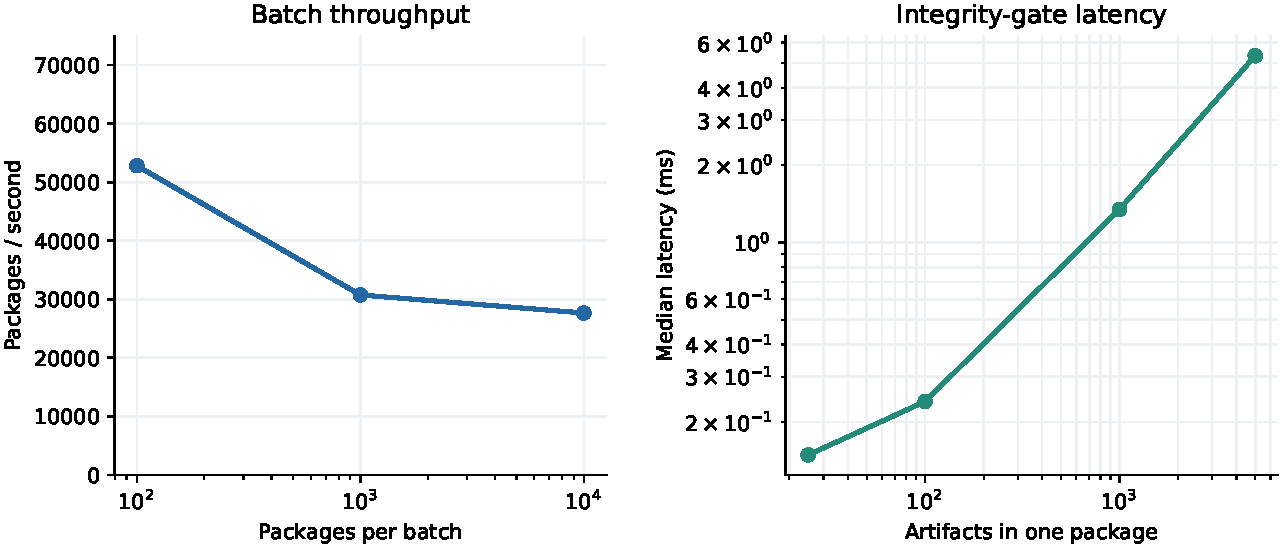
\includegraphics[width=0.98\textwidth]{Fig4.pdf}
\caption{MouseClaimBench component microbenchmarks on one Apple arm64 host using medians from five repetitions after warm-up. The left panel times local core authorization for batches of 100, 1,000, and 10,000 pristine packages. The right panel times the local integrity gate for one valid package containing 25, 100, 1,000, or 5,000 artifacts. Downloads, source predicates, graph serialization, and external \ac{shacl} execution are excluded. The measurements are not end-to-end throughput}
\label{fig:scalability-v2}
\end{figure}

%% END ORIGINAL SOURCE: scalability_v2.tex





%% BEGIN ORIGINAL SOURCE: scalability_results.tex (SHA256 d7525a73fd835ef16925fde5551da548a49a79f34eeaf9c4fbb72734a7dbebbc)
\begin{table}[!htbp]
\centering
\caption{MouseClaimBench component microbenchmarks on one Apple arm64 host. Every value is the median of five repetitions after warm-up. Downloads, source predicates, graph serialization, and external \ac{shacl} execution are excluded}
\label{tab:scalability-results}
\footnotesize
\renewcommand{\arraystretch}{1.05}
\begin{tabularx}{\textwidth}{@{}Y r r r@{}}
\toprule
Workload & Size & Median time (ms) & Throughput \\
\midrule
Evidence-package batch & 100 packages & 1.893 & 52,816 packages/s \\
Evidence-package batch & 1,000 packages & 32.529 & 30,742 packages/s \\
Evidence-package batch & 10,000 packages & 361.629 & 27,653 packages/s \\
Single digital-twin package & 25 artifacts & 0.149 & Not pooled \\
Single digital-twin package & 100 artifacts & 0.240 & Not pooled \\
Single digital-twin package & 1,000 artifacts & 1.344 & Not pooled \\
Single digital-twin package & 5,000 artifacts & 5.328 & Not pooled \\
\bottomrule
\end{tabularx}
\end{table}

%% END ORIGINAL SOURCE: scalability_results.tex



\FloatBarrier


\subsection{Artifact-grounded applications in computational neuroscience}
\label{subsec:application-results}

The artifact-grounded evaluation tests whether the same authorization
architecture produces bounded decisions when applied to heterogeneous public
mouse-brain evidence.

The retrospective mapping evaluates five bounded target claims and five
strict digital-twin claims. Applying profile v2 to the corresponding frozen
evidence packages authorizes bounded prediction for Static Sensorium,
topology-specific behavioral prediction for \ac{ibl}, and a local
observational structure--function association for \ac{microns}. Allen
directed topology lacks several mandatory evidence blocks, while Dynamic
Sensorium retains a response-reliability review state. The strict
entity-specific whole-brain digital-twin claim is not authorized for any
retrospective resource.

The dependence-aware \ac{microns} analysis updates the evidential status of
the local association without expanding its scientific scope.
Table~\ref{tab:microns-dyadic-results} reports cohort size, directed-pair
counts, effect estimates, uncertainty, and both inferential checks.

No permuted coefficient is at least as large as the observed positive
coefficient in any window. With 1,000 permutations, the finite-permutation
corrected value is therefore

\[
p=\frac{1}{1001}\approx0.001
\]

in each window. The discovery-window value remains descriptive because that
window fixed the positive direction. Both pre-fixed hold-outs satisfy the
positive-coefficient, two-sided dyadic, and one-sided permutation criteria.
Shared-neuron dependence is explicitly addressed rather than treating
directed neuron pairs as independent.

All windows nevertheless originate from one \ac{microns} volume, and
readout-location similarity is a derived functional descriptor rather than a
causal measurement. The authorized interpretation therefore remains a local
observational structure--function association.



%% BEGIN ORIGINAL SOURCE: microns_dyadic_results.tex (SHA256 1eb35195c3f40d5fa09751d1e9335d33fbe330171de9316192e6fb40ca62cfec)
\begin{table}[!htbp]
\centering
\caption{Dependence-aware \ac{microns} inference for the fixed all-pairs/readout-location endpoint. Candidate and connected counts refer to directed pairs. Confidence intervals use the same unit-based degrees of freedom as the directed dyadic test. Discovery fixes the positive direction, so its one-sided permutation value is descriptive. Confirmation requires $\widehat{\beta}>0$, two-sided $p_{\mathrm{dyadic}}\leq0.05$, and one-sided $p_{\mathrm{perm}}\leq0.05$ in both pre-fixed hold-outs}
\label{tab:microns-dyadic-results}
\scriptsize
\renewcommand{\arraystretch}{1.05}
\setlength{\tabcolsep}{2.5pt}
\begin{tabularx}{\textwidth}{@{}Y r r r r r r@{}}
\toprule
Cohort & Units & Pairs (connected) & $\widehat{\beta}$ (SE) & 95\% CI & $p_d$ & $p_p$ \\
\midrule
Discovery & 1,000 & 999,000 (2,095) & 0.0106 (0.00200) & [0.00668, 0.01451] & $1.39\times10^{-7}$ & 0.0010 \\
Hold-out 1 & 992 & 983,072 (1,926) & 0.0178 (0.00209) & [0.01372, 0.02192] & $5.78\times10^{-17}$ & 0.0010 \\
Hold-out 2 & 999 & 997,002 (1,922) & 0.0117 (0.00205) & [0.00763, 0.01569] & $1.76\times10^{-8}$ & 0.0010 \\
\bottomrule
\end{tabularx}
\end{table}

%% END ORIGINAL SOURCE: microns_dyadic_results.tex



The two frozen \ac{dandi} protocols produce opposite authorization outcomes.
DANDI:001176 fails the pre-specified availability requirement with 5 usable
subjects against a frozen minimum of 20. No predictive model is therefore
fitted.

DANDI:000039 yields 32 usable mice, a median held-out correlation of 0.310,
a mouse-bootstrap 95\% interval of $[0.207,0.369]$, and 93.75\% of mice with
positive held-out correlation. Model and intercept squared-error sums are
11.579 and 12.244 over 6,193 held-out trials, corresponding to a 5.43\%
relative reduction. All five frozen authorization conditions pass. The
result therefore authorizes only bounded population-response prediction.

A later audit confirms that every held-out contrast, direction, and joint
condition occurs in the training data for every mouse. The audit changes no
split, model, threshold, or authorization decision. Table~\ref{tab:dandi-threshold-sensitivity} reports a separate, post-outcome sensitivity analysis; it does not change the frozen protocols.



%% BEGIN ORIGINAL SOURCE: dandi_threshold_sensitivity.tex (SHA256 6fd3aa06a62327033f7ff1d7a3da0a5832bdc4feb7e7ece7375031de88c0cda6)
\begin{table}[!htbp]
\centering
\caption{Post-outcome, one-at-a-time sensitivity of the author-defined DANDI acceptance criteria. The frozen threshold is the prospective decision rule. The unit labels follow the corresponding frozen protocol and DANDI metadata. The last column reports the nearest tested decision boundary or, when no boundary is crossed, the observed outcome. It is not a recommended replacement or a criterion-valid standard}
\label{tab:dandi-threshold-sensitivity}
\scriptsize
\renewcommand{\arraystretch}{1.02}
\begin{tabularx}{\textwidth}{@{}Y r r P{0.34\textwidth}@{}}
\toprule
Criterion & Frozen & Observed & Sensitivity boundary or outcome \\
\midrule
DANDI:000039 usable mice & $\geq25$ & 32 & $\geq33$ \\
Median mouse correlation & $\geq0.10$ & 0.310 & $\geq0.35$ \\
Bootstrap lower bound & $>0$ & 0.207 & $>0.25$ \\
Positive-mouse fraction & $\geq0.65$ & 0.938 & $\geq0.95$ \\
Relative squared-error gain & $>0$ & 5.43\% & $>7.5\%$ \\
DANDI:001176 usable subjects (mice) & $\geq20$ & 5 &
Negative at every tested minimum $\geq10$ and available only at $\leq5$ \\
\bottomrule
\end{tabularx}
\end{table}
%% END ORIGINAL SOURCE: dandi_threshold_sensitivity.tex



The one-at-a-time sensitivity analysis leaves the frozen DANDI:000039
decision unchanged while making its finite decision margins explicit. The
decision would fail if the required number of mice were increased to 33, the
median-correlation threshold to 0.35, the bootstrap lower-bound threshold to
0.25, the positive-mouse fraction to 0.95, or the required squared-error
improvement to 7.5\%.

DANDI:001176 remains unavailable for every tested minimum of at least 10
subjects and would satisfy the availability requirement only after the
prohibited relaxation to five subjects. These post-outcome sensitivity
experiments expose the location of the decision boundaries and do not provide
criterion validation for the thresholds. Fig.~\ref{fig:prospective-applications-v2} displays the two opposite prospective DANDI outcomes.



%% BEGIN ORIGINAL SOURCE: prospective_applications_v2.tex (SHA256 fc3d6cbf70034bb3d39238deaf218fafe4cfd423a4d6d49daf4fdb9a83779d36)
\begin{figure}[!htbp]
\centering
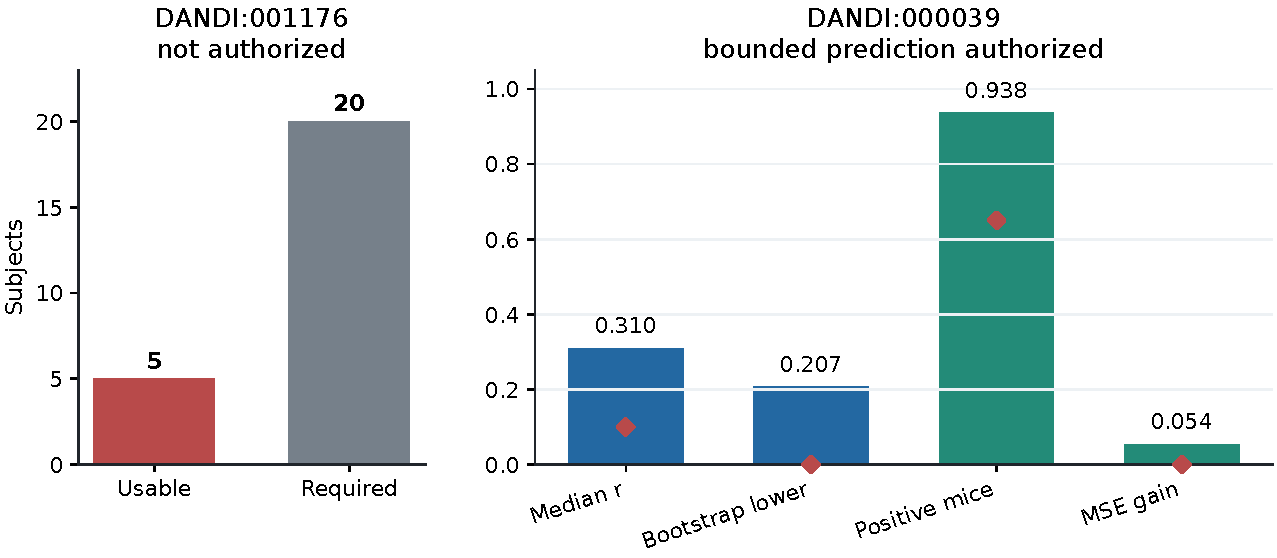
\includegraphics[width=0.90\textwidth]{Fig5.pdf}
\caption{Prospective DANDI outcomes under rules fixed before numerical asset access. DANDI:001176 provides 5 usable subjects against the predeclared minimum of 20, so no model is fitted. DANDI:000039 passes every frozen condition across 32 mice, with median held-out correlation 0.310, mouse-bootstrap lower bound 0.207, 93.8\% positive mice, and relative MSE reduction 0.054. Red diamonds mark the respective thresholds of 0.10, 0, 0.65, and 0. Bar heights are criterion-specific values and are not intended for direct cross-metric comparison. Only bounded population-response prediction is authorized}
\label{fig:prospective-applications-v2}
\end{figure}

%% END ORIGINAL SOURCE: prospective_applications_v2.tex



\FloatBarrier

The positive DANDI result is not presented as a state-of-the-art predictive
model. Ridge regression was intentionally fixed because the experiment tests
prospective claim authorization rather than neural-architecture performance.
The availability refusal is equally informative for the system evaluation.

Together, the two frozen protocols demonstrate that the same executable
knowledge contract can preserve both authorization and refusal without
post-outcome modification of endpoints or thresholds. The later sensitivity
analysis cannot alter either frozen decision. The final release additionally
verifies source revisions, profile and protocol hashes, exact public DANDI
asset identifiers, and the absence of \texttt{-dirty} artifacts. Table~\ref{tab:prospective-applications} summarizes these and the retrospective bounded application decisions without extending their scope.



%% BEGIN ORIGINAL SOURCE: prospective_applications.tex (SHA256 4c32e545a96dfb4121696257369b8eabc1828099871a3657f46e31f2aa840477)
\begin{table}[H]
\centering
\caption{Artifact-grounded and prospective mouse-brain decisions. Authorization never extends beyond the claim stated in the second column}
\label{tab:prospective-applications}
\footnotesize
\renewcommand{\arraystretch}{1.08}
\begin{tabularx}{\textwidth}{@{}P{0.17\textwidth}P{0.23\textwidth}P{0.10\textwidth}Y@{}}
\toprule
Resource & Bounded target claim & Decision & Decisive result or deficit \\
\midrule
Allen \ac{vbn} & Directed topology and prediction & No & Topology and direction fail, with further missing blocks \\
Static Sensorium & Bounded predictive performance & Yes & Five-dataset comparison passes declared prediction and quality rules \\
Dynamic Sensorium & Bounded predictive performance & No & Response reliability requires review \\
IBL & Topology-specific behavioral prediction & Yes & Locked two-split comparison passes, without exclusive superiority \\
\ac{microns} & Local structure--function association & Yes & Direction fixed in discovery. Both pre-fixed hold-outs pass dyadic and node-label permutation criteria \\
DANDI:001176 & Cortical \ac{ach} prediction & No & 5 usable subjects against a frozen minimum of 20 \\
DANDI:000039 & Population contrast-response prediction & Yes & 32 mice, median $r=0.310$, bootstrap lower bound 0.207 \\
Strict digital twin & Entity-specific whole-brain twin & No & Zero authorizations across all evaluated resources \\
\bottomrule
\end{tabularx}
\end{table}

%% END ORIGINAL SOURCE: prospective_applications.tex


%% END ORIGINAL SOURCE: experiments.tex



%% BEGIN ORIGINAL SOURCE: discussion.tex (SHA256 18135e7663bf2084fb5e88fe796b6ad643e7a2578de00e5805e0623ad959262a)
\section{Discussion}
\label{sec:discussion}

The results support MouseClaimBench as an integrity-aware intelligent system
for scientific claim authorization over heterogeneous evidence packages.
Its central behavior is non-compensatory: evidence that is admissible for one
claim cannot silently justify another claim with different evidential
requirements, and structural correctness or provenance completeness cannot
substitute for missing scientific evidence. Authorization remains explicitly
relative to a versioned knowledge profile, while refusal preserves the
complete set of detected deficit categories and their corresponding
witnesses.

The evaluation provides evidence at several complementary levels. The
reasoning implementation conforms to the declared authorization semantics
across separately implemented execution paths; counterfactual experiments
support the fidelity of the explanation mechanism; controlled attacks
characterize the behavior of the integrity layer and its trust boundary; and
artifact-grounded applications show that the same executable knowledge
contract can retain both authorization and refusal when applied to public
computational-neuroscience resources. These results establish the behavior of
the proposed authorization architecture without equating successful
authorization with scientific truth.


\subsection{Scientific interpretation and methodological contribution}
\label{subsec:interpretation-novelty}

The primary methodological contribution is the formulation and executable
realization of scientific claim authorization as a distinct intelligent-system
decision problem. The system does not ask only whether a document supports a
statement, whether a graph satisfies a structural schema, or whether a model
passes an isolated validation metric. Instead, it reasons over whether a
heterogeneous evidence package satisfies the complete scientific, structural,
and integrity requirements associated with a bounded claim under an explicit
knowledge profile.

This formulation separates three types of reasoning that are often conflated
in evidence-based computational workflows. Domain authorization concerns the
scientific admissibility of claim-specific evidence. Structural conformance
concerns the correctness and completeness of its representation. Package
integrity concerns relational consistency across provenance, artifact
identity, attestations, cohort declarations, and independence claims. The
final decision combines these dimensions through
$S\land A\land I^{\mathrm{clean}}$, while retaining their deficit traces
independently. This separation allows the system to distinguish, for example,
a scientifically failed but structurally well-formed package from an
otherwise sufficient package whose provenance relations are inconsistent.

The use of \ac{shacl}, \ac{prov}, JSON-LD, Python, and \ac{asp} is not itself
the methodological novelty. These technologies provide complementary
representation, validation, and reasoning mechanisms within the proposed
architecture. The contribution lies in defining the scientific authorization
problem, assigning explicit semantics to its evidence and deficit states, and
executing the resulting non-compensatory decision model across independently
scoped reasoning paths. In this sense, MouseClaimBench extends the traditional
expert-system separation between knowledge representation, facts, inference,
and explanation to heterogeneous scientific evidence packages with explicit
integrity requirements.

The conformance results support this interpretation. Python and the
separately implemented \ac{asp} path agree on all domain decisions and
deficit sets, while external \ac{shacl} validation reproduces the expected
structural behavior without acting as a scientific authorization engine.
The eight-state final-gate evaluation confirms that successful authorization
requires simultaneous satisfaction of structural, domain, and integrity
conditions rather than success in any individual layer.

The one-edge perturbation experiment further characterizes the local
sensitivity of the symbolic decision policy. Fifty-nine relation removals are
not individually decisive because other deficits remain, whereas removing the
\texttt{data\_quality} relation from bounded prediction changes the Dynamic
Sensorium decision. Conversely, adding currently unprovided requirements
produces 71 authorization contractions. These results are consistent with the
expected monotonic behavior of the non-compensatory model and identify which
relations are decision-critical in the fixed packages. They do not establish
that alternative profiles are scientifically preferable.

The explanation results provide a second level of validation. Repairing all
reported deficits restores authorization in every one of the 9,839
non-authorized generated packages, and restoring each repaired deficit
individually produces 51,480 successful necessity checks. The explanation
mechanism therefore preserves the requirements that are causally relevant to
the authorization decision under the declared symbolic semantics. The
41,641 deficit records that would be omitted by a single-reason baseline
quantify the information retained by category-complete reporting. This
demonstrates explanation fidelity to the implemented reasoning contract, not
perceived usefulness to human reviewers.


\subsection{Integrity reasoning and explicit trust boundaries}
\label{subsec:integrity-discussion}

The integrity experiments show why provenance representation alone is
insufficient for claim authorization. Under the controlled threat model, the
complete domain-plus-integrity configuration rejects all 2,550 attacked
packages spanning every non-empty composition of the eight historical attack
families. The extended regression suite and direct API tests further cover
reference closure, attestation consistency, duplicate declarations, reflexive
relations, and composite generation identity.

The leave-one-control-out results distinguish essential controls from
defensive overlap. Removing seven individual controls introduces false
authorization in the corresponding single-attack cases, while removal of the
contradictory-attestation check is masked by the independently active
block--attestation consistency control. This behavior is desirable in a
defense-in-depth setting because multiple checks may constrain the same
invalid package through different invariants.

The 20 internally coherent forgery controls expose a different limitation.
Packages whose false content, hashes, or independence metadata remain
internally self-consistent cannot be rejected solely through internal
reasoning. MouseClaimBench therefore provides integrity reasoning over
declared evidence relations rather than source authentication. External trust
anchors such as signed attestations, trusted repositories, or independently
verifiable identities would be required to move that boundary outward.

This distinction is important for intelligent systems operating over
scientific artifacts. An auditable reasoning architecture should make explicit
not only what it can reject but also which classes of deception are
indistinguishable from valid inputs under its information model. The coherent
forgery controls therefore serve as an explicit characterization of the
system's trust boundary rather than as failed attack detections.


\subsection{Artifact-grounded scientific interpretation}
\label{subsec:artifact-interpretation}

The computational-neuroscience applications illustrate how the authorization
architecture behaves when its evidence predicates are grounded in real public
resources. The retrospective cases preserve bounded distinctions among
prediction, topology-specific behavior, local structure--function association,
and strict digital-twin claims. In particular, successful evidence for one
bounded target does not propagate into authorization of the complete
entity-specific digital-twin claim.

The two frozen \ac{dandi} protocols provide complementary prospective
outcomes. DANDI:001176 preserves a refusal because only 5 usable subjects
satisfy the frozen schema against a required minimum of 20. No predictive
model is fitted after this failure. DANDI:000039 instead satisfies all five
pre-specified requirements across 32 mice and therefore authorizes only the
bounded population-response prediction defined by the profile. The use of a
simple ridge model is deliberate: the experiment evaluates whether a frozen
authorization contract preserves its decision rules after data access rather
than whether a new predictive architecture achieves state-of-the-art
performance.

The post-outcome sensitivity analysis clarifies the finite margins around the
DANDI decisions without changing them. DANDI:000039 would fail under stricter
thresholds for sample size, median correlation, bootstrap lower bound,
positive-mouse fraction, or squared-error improvement, while DANDI:001176
would become available only after relaxing the frozen sample requirement to
five subjects. These analyses therefore expose the decision boundary of the
declared profile rather than retroactively calibrating its thresholds.

The dependence-aware \ac{microns} analysis provides a different form of
artifact-grounded evidence. Directed dyadic covariance and simultaneous
node-label permutations address dependence induced by shared neurons, and
both pre-fixed hold-outs satisfy the declared inferential requirements after
the positive direction is fixed in discovery. The authorized interpretation
nevertheless remains a local observational structure--function association.
One cortical volume does not establish external biological replication,
causality, or complete visual-cortex coverage.

Taken together, these applications illustrate the practical role of
claim-specific authorization: the same reasoning architecture can preserve
positive, negative, and deliberately bounded outcomes without converting
successful evidence into a broader scientific conclusion.


\noindent\textbf{Lessons learned.}\label{par:lessons-learned}\par

Five practical lessons emerge from the evaluation. First, structural
conformance should be delegated to a standard validation mechanism rather
than conflated with domain reasoning. Second, provenance should represent
dependence and independence assertions, not only artifact locations and
derivations. Third, negative outcomes should remain first-class release
artifacts because refusal is part of the intelligent-system behavior rather
than an experimental failure. Fourth, explanation should preserve all
decision-relevant deficit categories instead of only one prioritized reason.
Finally, internal integrity reasoning requires an explicit trust boundary:
self-consistent false metadata cannot be distinguished from valid metadata
without an external source of trust.


\subsection{Limitations and threats to validity}
\label{subsec:limitations}

The principal construct-validity limitation concerns the content of the
authorization profile rather than the execution semantics of the system.
Profile v2 is author-defined and literature-grounded, with inspectable claims,
predicate contracts, claim--evidence relations, rationales, exceptions, and
sources. No independent panel has yet established the necessity, sufficiency,
or completeness of these profile requirements, and no eligible independent
rater has completed the frozen 92-item external content-validity protocol.
Accordingly, the reported authorization decisions are valid relative to the
declared profile rather than evidence of scientific consensus.

Internal validity is strongest for the implemented reasoning behavior.
Expected mutation, counterfactual, and integrity outcomes are defined by the
declared semantics, and agreement between multiple execution paths reduces
implementation-specific risk. However, Python and \ac{asp} share the same
profile specification, one-edge variants characterize only local policy
changes, property-based tests cover finite generated packages, and the attack
generator evaluates declared rather than adaptive threats. Internally
coherent false metadata remains outside the detectable integrity boundary
without external authentication.

The artifact-grounded applications are heterogeneous and should not be
interpreted as independent biological replications of one common hypothesis.
Five retrospective packages originate from MouseBrainBench
(\MouseBrainBenchCompanion). The \ac{microns} windows belong
to one tissue volume, while the two \ac{dandi} studies address different
measurements and decision questions. DANDI:000039 evaluates bounded
prediction rather than model superiority, and DANDI:001176 evaluates
resource availability under a frozen schema. Mouse-level bootstrap and
dyadic covariance address the declared dependence structures but retain their
respective exchangeability assumptions. The hold-outs and frozen Git
protocols provide temporal controls but were not registered in an external
preregistration service.

External validity has been demonstrated only within computational
mouse-brain evidence. The architecture supports alternative profiles, but
loading another profile establishes extensibility rather than empirical
cross-domain generality. Evaluation in other scientific domains would be
needed to determine how well the authorization abstraction transfers to
different evidence types, claim vocabularies, and integrity requirements.

Human-centered evaluation also remains outside the present study.
Category-complete deficits are counterfactually faithful to the symbolic
decision process, but their comprehensibility, usefulness, and effect on
scientific decision making have not been evaluated with end users.

Finally, the performance study characterizes component-level execution on one
host. It excludes data access, source-predicate execution, graph
serialization, and external \ac{shacl} processing and should therefore not be
interpreted as an end-to-end scalability benchmark or portable latency
guarantee.
%% END ORIGINAL SOURCE: discussion.tex



%% BEGIN ORIGINAL SOURCE: conclusions.tex (SHA256 10d87e1b34a6a931702a018cc3bcedf55afd0d91dc20b60d12d676bf1b3182ec)
\section{Conclusions and Future Work}
\label{sec:conclusions}
MouseClaimBench provides an integrity-aware intelligent system for authorizing bounded scientific claims from heterogeneous evidence. Its central principle is non-compensation: predictive performance, reproducible execution, structural conformance, or provenance integrity cannot substitute for the scientific evidence required by a particular claim. Each authorization decision is tied to a versioned knowledge profile and preserves every violated requirement with an actionable witness.

The evaluation supports this behavior across complementary reasoning and validation layers. Python and the separately implemented \ac{asp} path agree on domain authorization, external \ac{shacl} validation recovers the expected structural outcomes, and property-based and counterfactual tests confirm the declared authorization semantics and explanation fidelity. The integrity evaluation blocks all 2,550 attacked packages under the evaluated attack families, while the 20 internally coherent forgeries expose the need for external trust anchors.

The artifact-grounded applications preserve the same distinction. The frozen \ac{dandi} protocols retain both refusal and bounded predictive authorization without post-access changes to their decision rules, while dependence-aware \ac{microns} inference supports a local observational structure--function association in two pre-fixed hold-outs. In all cases, authorization remains limited to the bounded claim whose complete evidence contract is satisfied.

Future work requires independent profile assessment, human evaluation of category-complete traces, signed attestations, adaptive attacks, externally registered protocols, and evaluation in additional scientific domains. Until these extensions are evaluated, MouseClaimBench supports a narrower but reproducible conclusion: heterogeneous scientific evidence can be authorized through an explicit symbolic contract without allowing success in one requirement to compensate for missing or incoherent evidence in another.
%% END ORIGINAL SOURCE: conclusions.tex


\section*{Statements and Declarations}
\subsection*{Competing interests}
\label{sec:competing-interest}

The authors declare no known competing financial interests or personal
relationships that could have appeared to influence the work reported in
this paper.

\subsection*{Author contributions}
\label{sec:credit}

\noindent
Alberto Fern\'andez-Isabel:
Conceptualisation, Methodology, Software, Investigation, Data curation,
Writing--original draft, Writing--review and editing.
\par

\noindent
Isaac Mart\'in de Diego:
Validation, Formal analysis, Investigation, Writing--original draft,
Writing--review and editing, Project administration.
\par

\noindent
Rub\'en Fuentes-Fern\'andez:
Methodology, Validation, Writing--original draft, Writing--review and editing.

\subsection*{Data and code availability}
\label{sec:data-code-availability}
The source code, knowledge profiles, tests, frozen protocols, lightweight
result artifacts, and manuscript are maintained in the public MouseClaimBench
repository at
\url{https://github.com/Fiutten/MouseClaimBench}.
The software snapshot used for the experiments reported in this work is
released as tag \texttt{v0.12.6} at
\url{https://github.com/Fiutten/MouseClaimBench/tree/v0.12.6}.
Each regenerated result artifact records the clean source commit used for its
execution. Raw Allen, Sensorium, IBL, MICRONS, and DANDI data remain governed
by their providers and are not redistributed. The prospective artifact
manifests retain public identifiers, versions, sizes, and official hashes.
Every reported result is linked to a recorded Git revision, and artifacts
marked as dirty are excluded from the release gate. A persistent DOI has not
been assigned, so the repository and tagged commit are reported without
implying DOI-backed archival permanence.

\subsection*{Funding}
\label{sec:funding}

This work was supported by the Spanish MICIU under the PID program in the
XMIDAS project [PID2021-122640OB-I00]. The funder had no role in study design,
data collection, analysis or interpretation, manuscript preparation, or the
decision to submit the article for publication.


\subsection*{Ethics approval and consent}
No new experiments involving human or animal subjects were undertaken as part of this study. The computational analyses use existing public research resources; responsibility for the original data collection and its applicable approvals remains with the respective data providers. Consent for publication is not applicable to this manuscript.

\setlength{\bibsep}{2pt}
\bibliographystyle{unsrtnat}
\bibliography{references}
\end{document}
